% Chapter Template

\chapter{2-D Memristor Simulation} % Main chapter title

\label{Chapter6} % Change X to a consecutive number; for referencing this chapter elsewhere, use \ref{ChapterX}

\lhead{Chapter 6. \emph{Memristor Simulation}} % Change X to a consecutive number; this is for the header on each page - perhaps a shortened title
\begin{doublespace}

Even though 1-D simulation is able to capture the main characteristics of the memristor it is still lacking certain physical effects that can be captured in a 2-D simulation such as the movement of ions inside the electrolytic solution which cancels some applied electric field. This chapter shows the simulation of a memristor in 2-D and compares the results with 1-D simulations. It starts with the simulation of a memristor with different PEDOT:PSS layer thicknesses and shows the changes in particle density distributions, electric field and current density. 
Transient simulations with a pulse train and a sinusoidal potentials are presented and compared to 1-D siumlations. Finally current vs time and I-V curves for an actual memristor are used to show the accuracy of 2-D simulations in capturing the behavior of the actual device .  

\section{Effect of PEDOT:PSS Thickness}

The physical dimensions of the memristor is presented in the previous chapter. Thickness of the PEDOT:PSS layer is very small compared to the other dimensions of the device such as the thickness of the electrolyte and length of the conductive material. This complicates the simulation of the PEDOT:PSS strip using a uniform mesh. Although non uniform meshing seems like an appropriate solution, a close examination of the numerical limitations show that this is not the case. Decreasing the mesh size in one dimension severely reduces the maximum time step for the entire simulation therefore non uniform meshing is not feasible for this problem. 

An alternative solution to the meshing problem is using an infinitesimally thin PEDOT:PSS layer in a 2-D simulation. This method is used for the memristor simulations in this chapter. For PEDOT:PSS, the effects in 2-D are ignored since the layer thickness is 10000 times smaller than other dimensions such as the thickness of the electrolyte. For holes in the conductive layer only the horizontal component of the electric field is used and all the current densities are calculated in 1-D. Following plots compare two simulations with PEDOT:PSS thicknesses higher than the actual device thicknesses and a 2-D simulation with 1-D PEDOT:PSS layer.  

\begin{figure}[!htp]
\centering
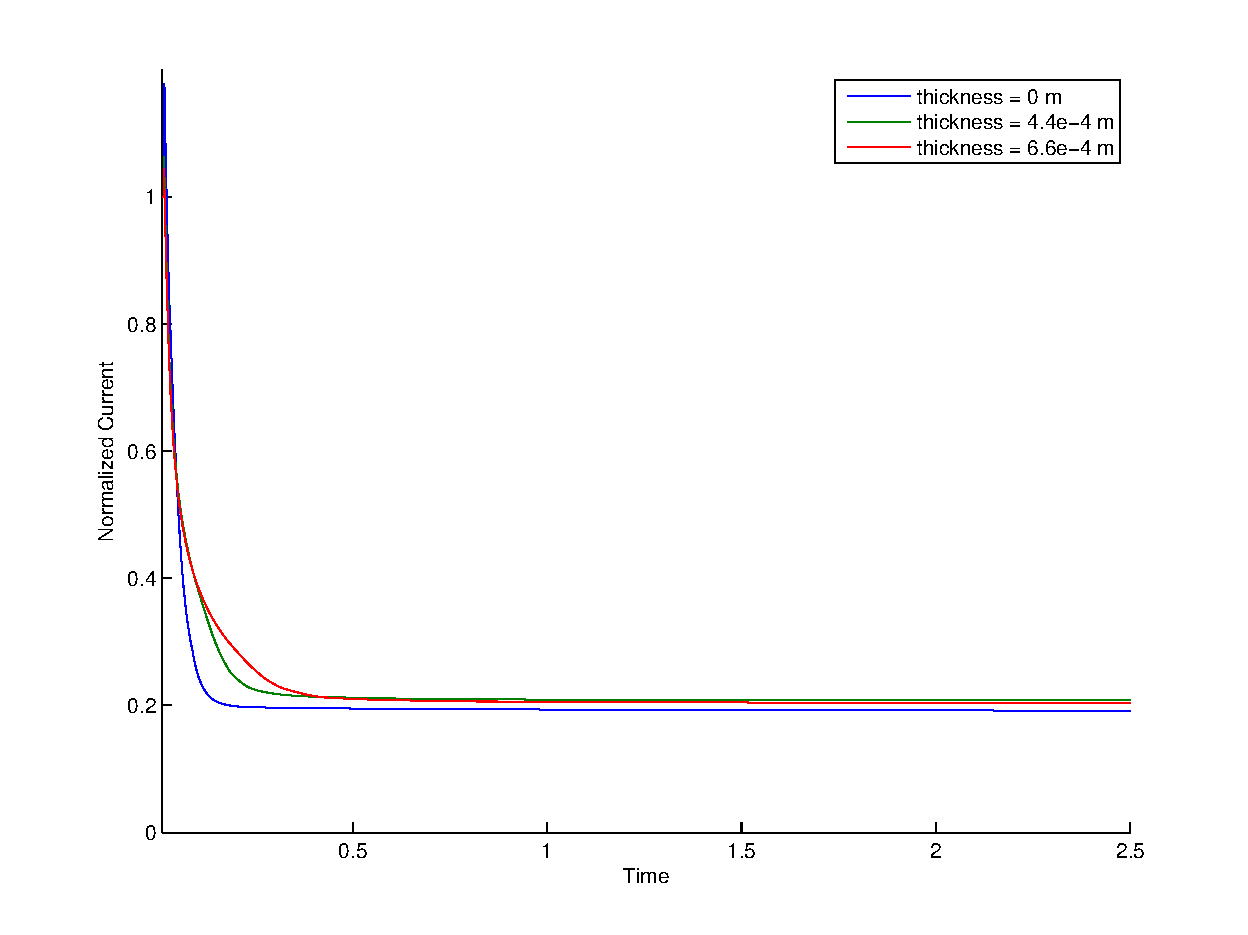
\includegraphics[scale=0.45]{2D_Memristor_Thick_Resistivity}
\caption{} 
\label{thick_resistivity}
\end{figure}

The memristor is simulated using a constant potential at the contacts. Left metal contact is 1 V and the right metal contact is grounded. Resistivity measured at the right contact for different PEDOT:PSS thicknesses is shown in figure \ref{thick_resistivity}. Resistivity plots show that as the thickness gets smaller the device responds faster. This is due to the decrease in the distance lithium ions have to travel inside PEDOT:PSS in order to change its resistivity. Another change in the behavior of the memristor is its resistivity at steady state. The increase in resistivity for different thicknesses at steady state can be attributed to the ion/hole interaction at the interface between PEDOT:PSS and electrolyte solution which is illustrated in the following figures \ref{thick_p_ss}, \ref{thick_li_ss} and \ref{thick_perch_ss}.

\begin{figure}[!htp]
\centering
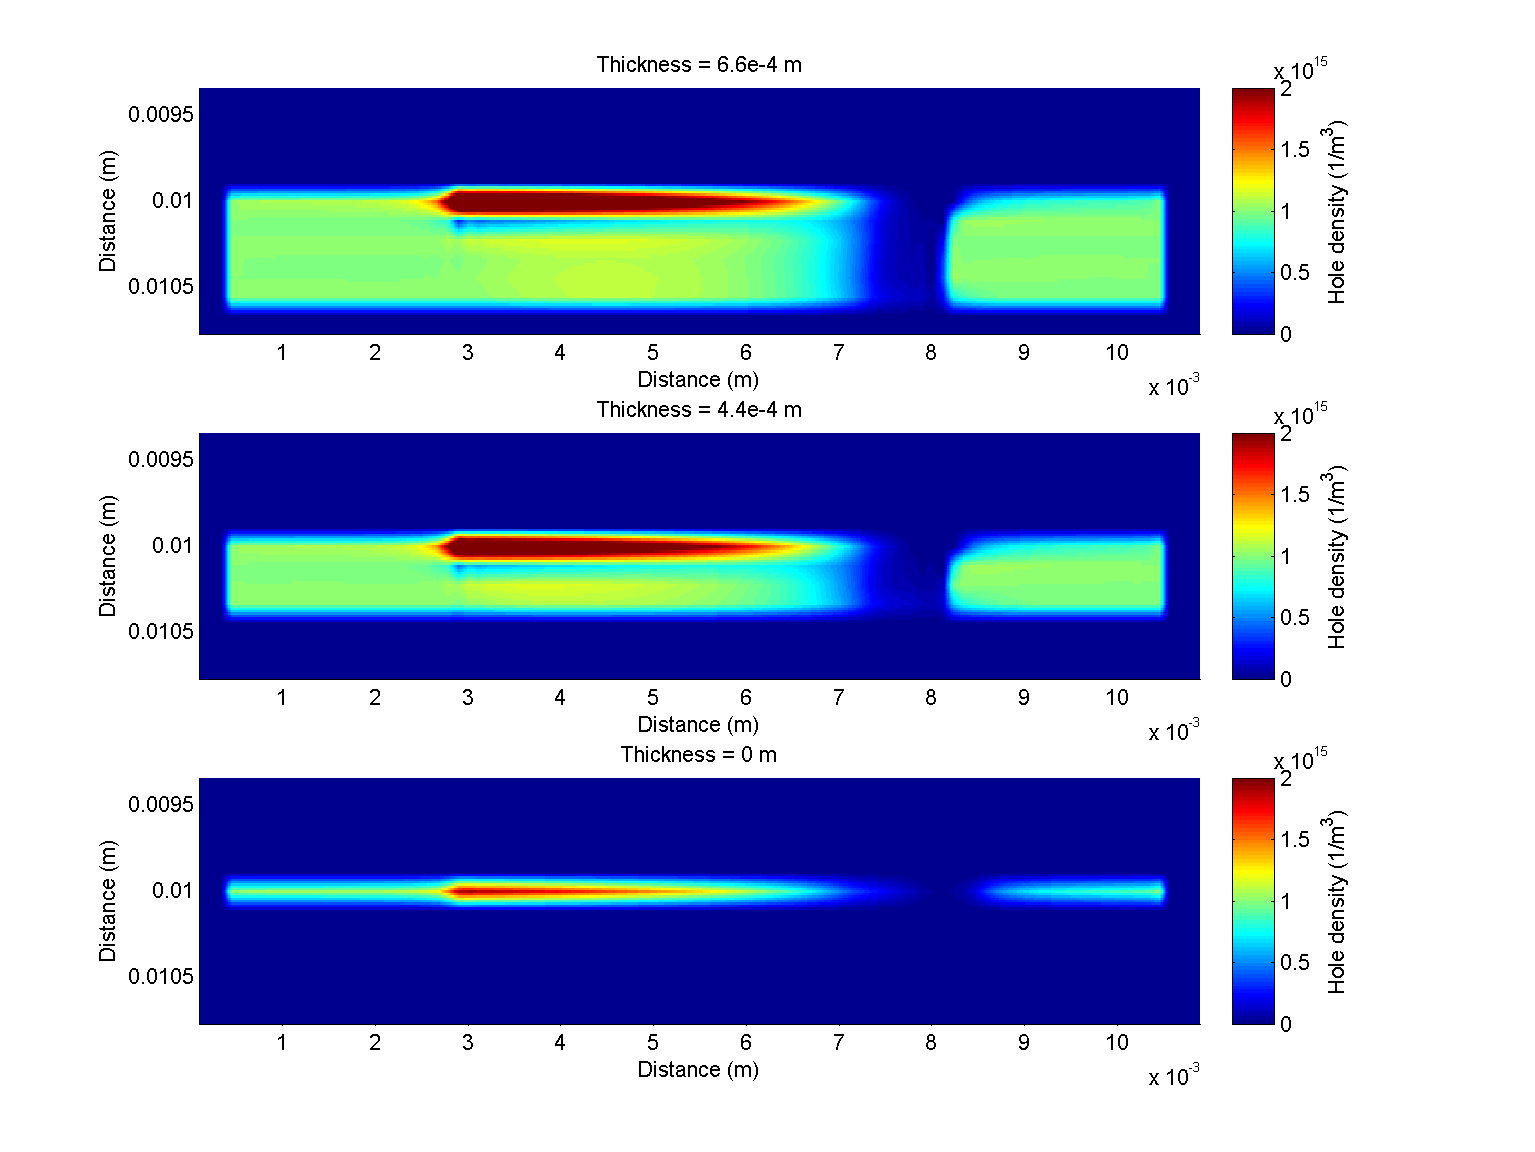
\includegraphics[scale=0.50]{2D_Memristor_Thick_Hole_SS}
\caption{} 
\label{thick_p_ss}
\end{figure}


Figure \ref{thick_p_ss} shows the hole distribution in PEDOT:PSS at steady state for different thicknesses. The electrolyte is on top of PEDOT:PSS but it is not visible in these plots since its hole concentration is zero at all times. As lithium ions move into the PEDOT:PSS they move towards the negative contact and push the holes out. This effect can be seen in figures \ref{thick_p_ss} and  \ref{thick_li_ss}. For all the plots, there is a section of the hole distribution which is missing due to lithium ions.

\begin{figure}[!htp]
\centering
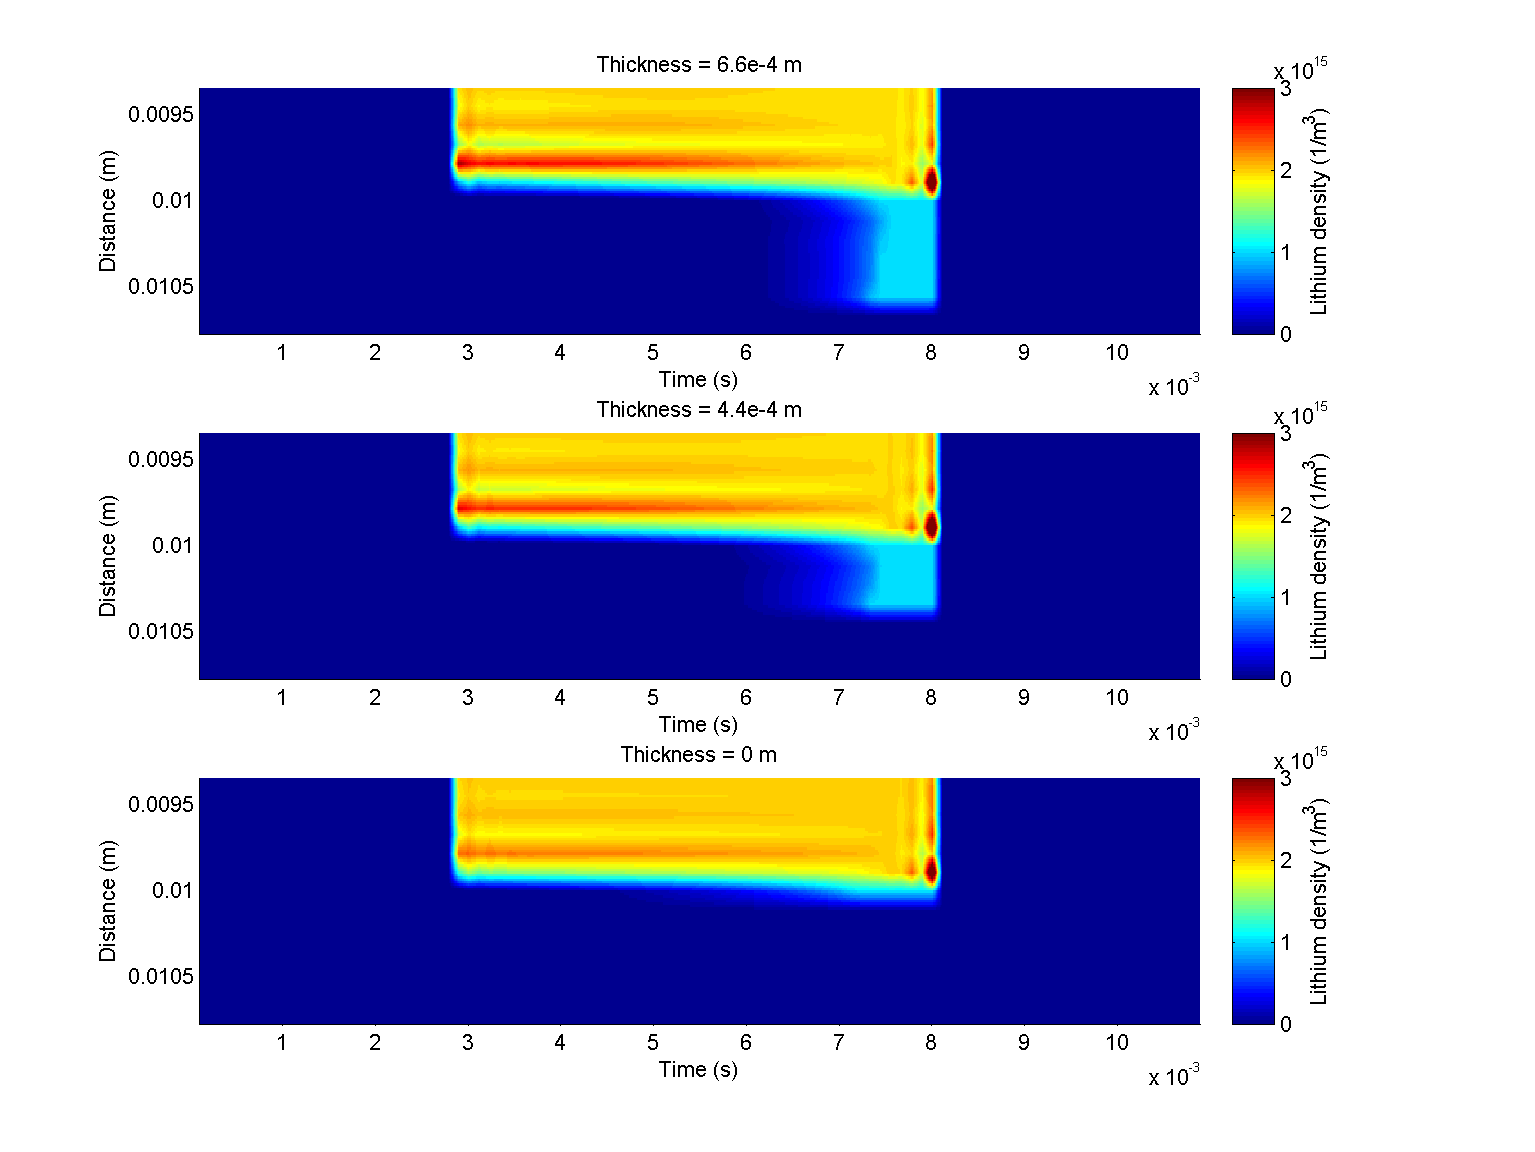
\includegraphics[scale=0.50]{2D_Memristor_Thick_Lithium_SS}
\caption{} 
\label{thick_li_ss}
\end{figure}

The accumulation of holes at the surface of the PEDOT:PSS is due to the perchlorate accumulation near the positive contact in the electrolyte (figure \ref{thick_perch_ss}). As perchlorate ions accumulate on the surface of the PEDOT:PSS they also attract holes towards the surface.

\begin{figure}[!htp]
\centering
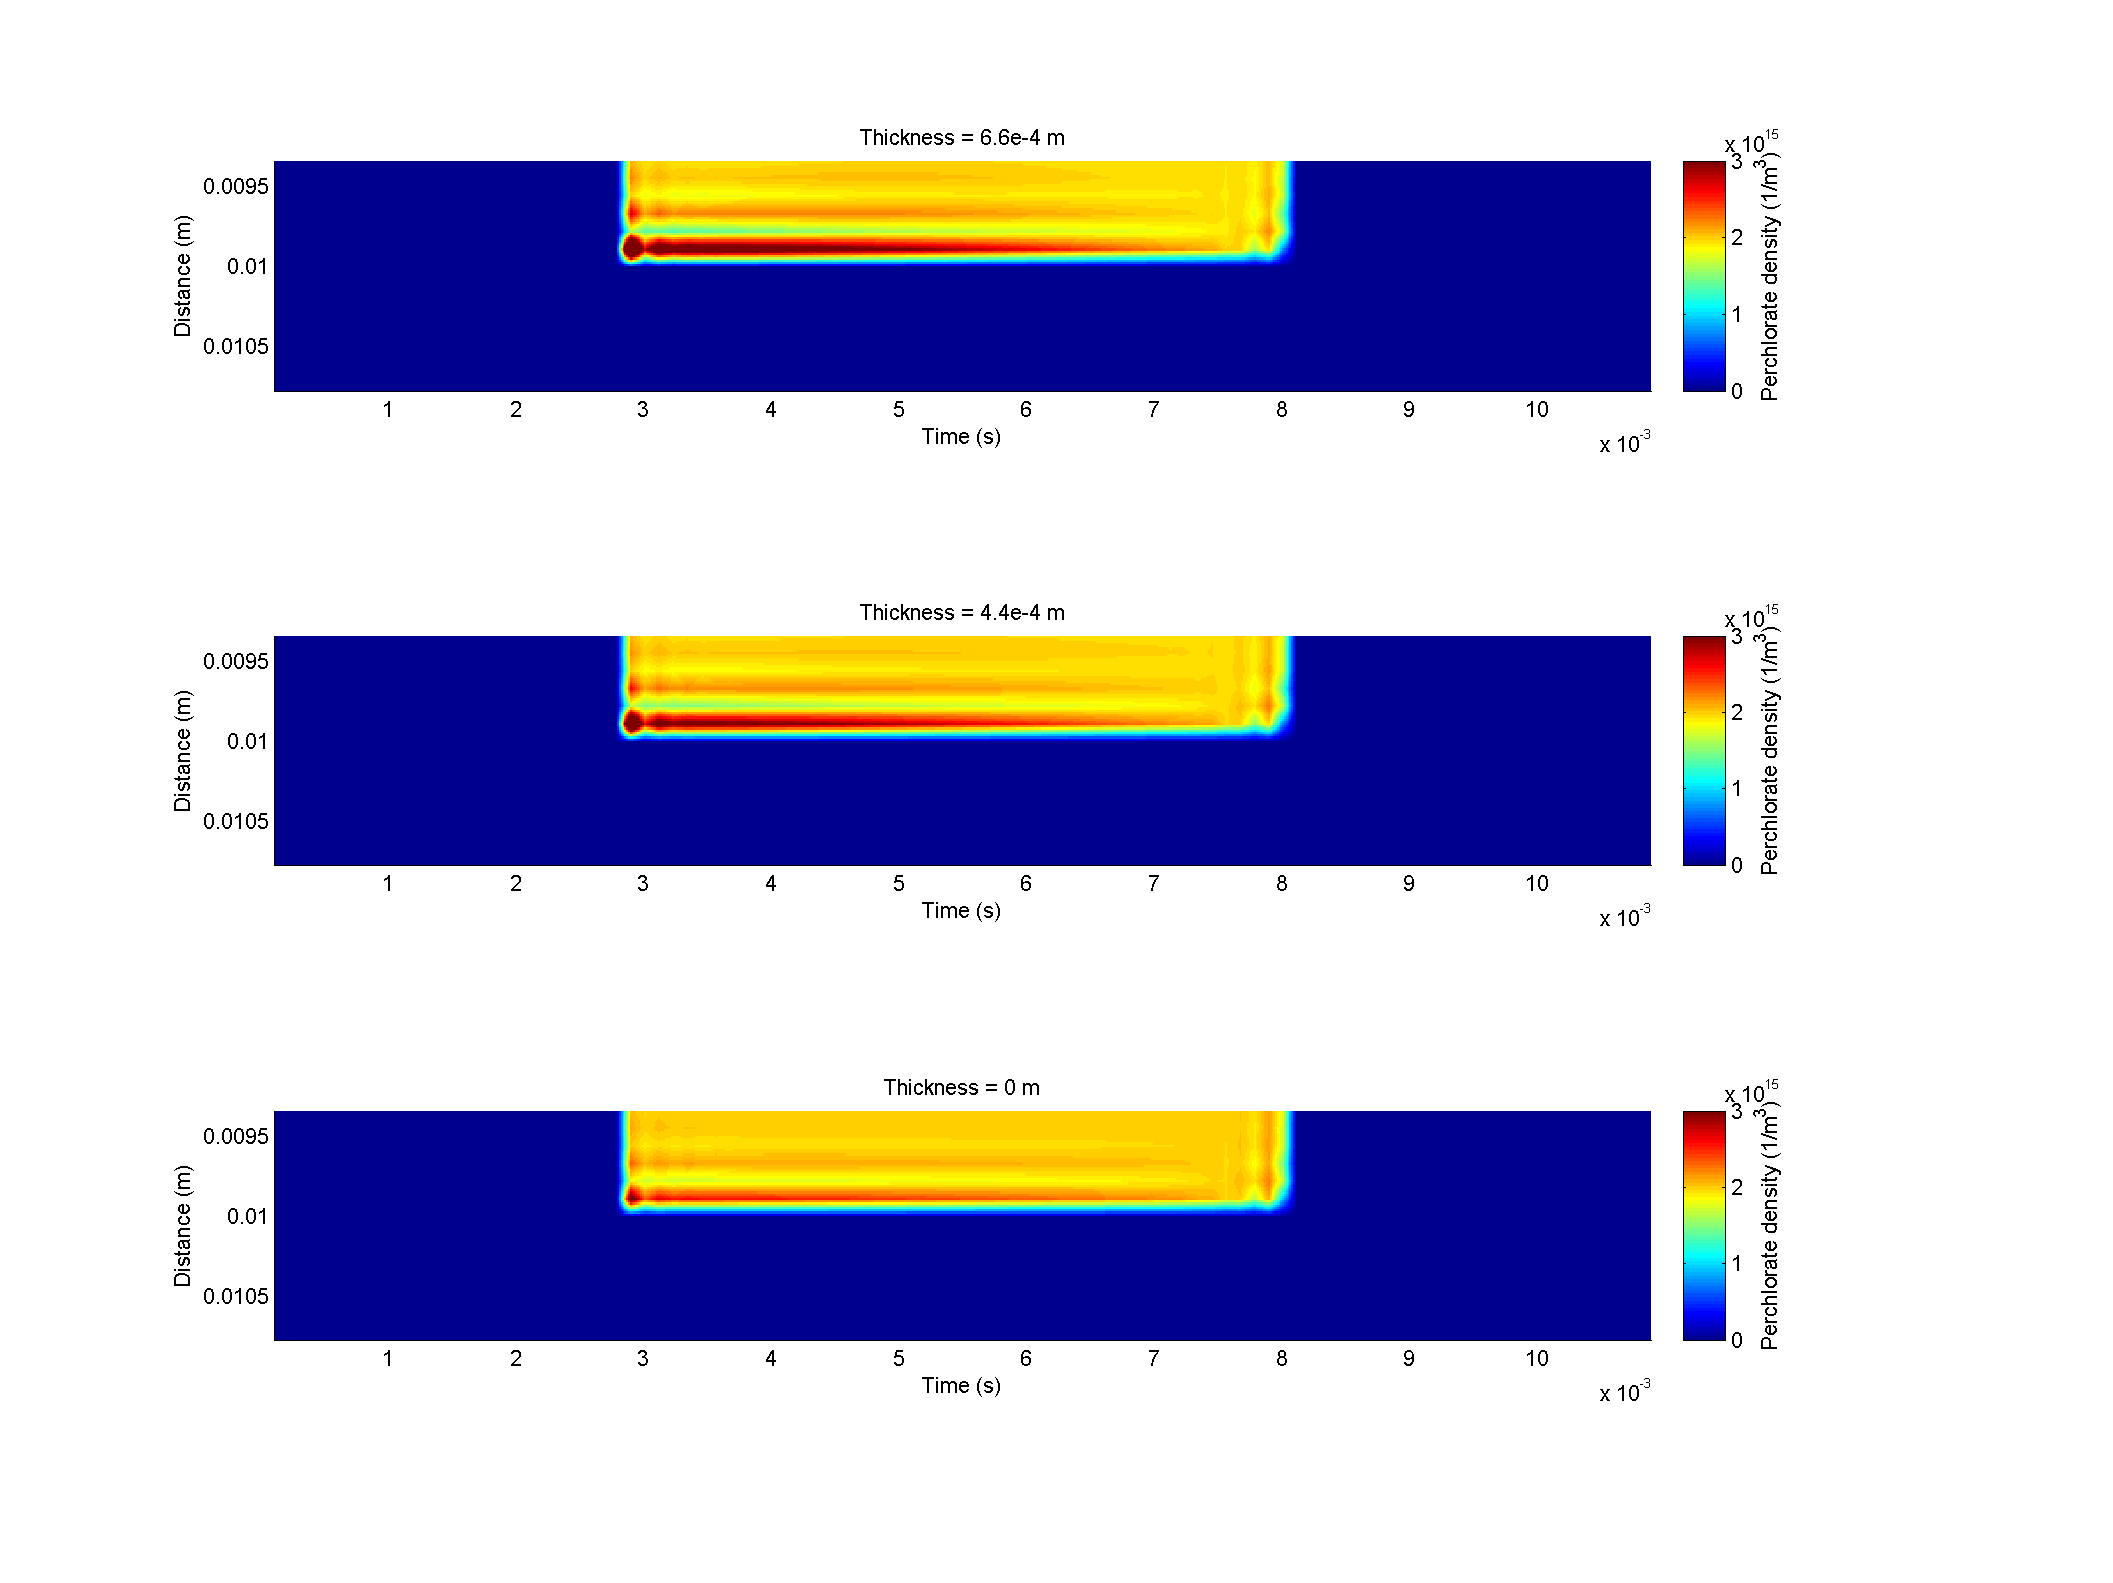
\includegraphics[scale=0.40]{2D_Memristor_Thick_Perchlorate_SS}
\caption{} 
\label{thick_perch_ss}
\end{figure}

Figure \ref{thick_netq_p} shows the charge density of holes at the surface of the PEDOT:PSS and the net charge density in the electrolyte near PEDOT:PSS. Negative charges that accumulate on the left side of the electrolyte attract holes and positive charges on the right side push them out. This additional mechanism is the key difference between 1-D and 2-D simulations. In 1-D simulation, ion density inside the electrolyte and the changes in the electric field due to these charges were not present.

\begin{figure}[!htp]
\centering
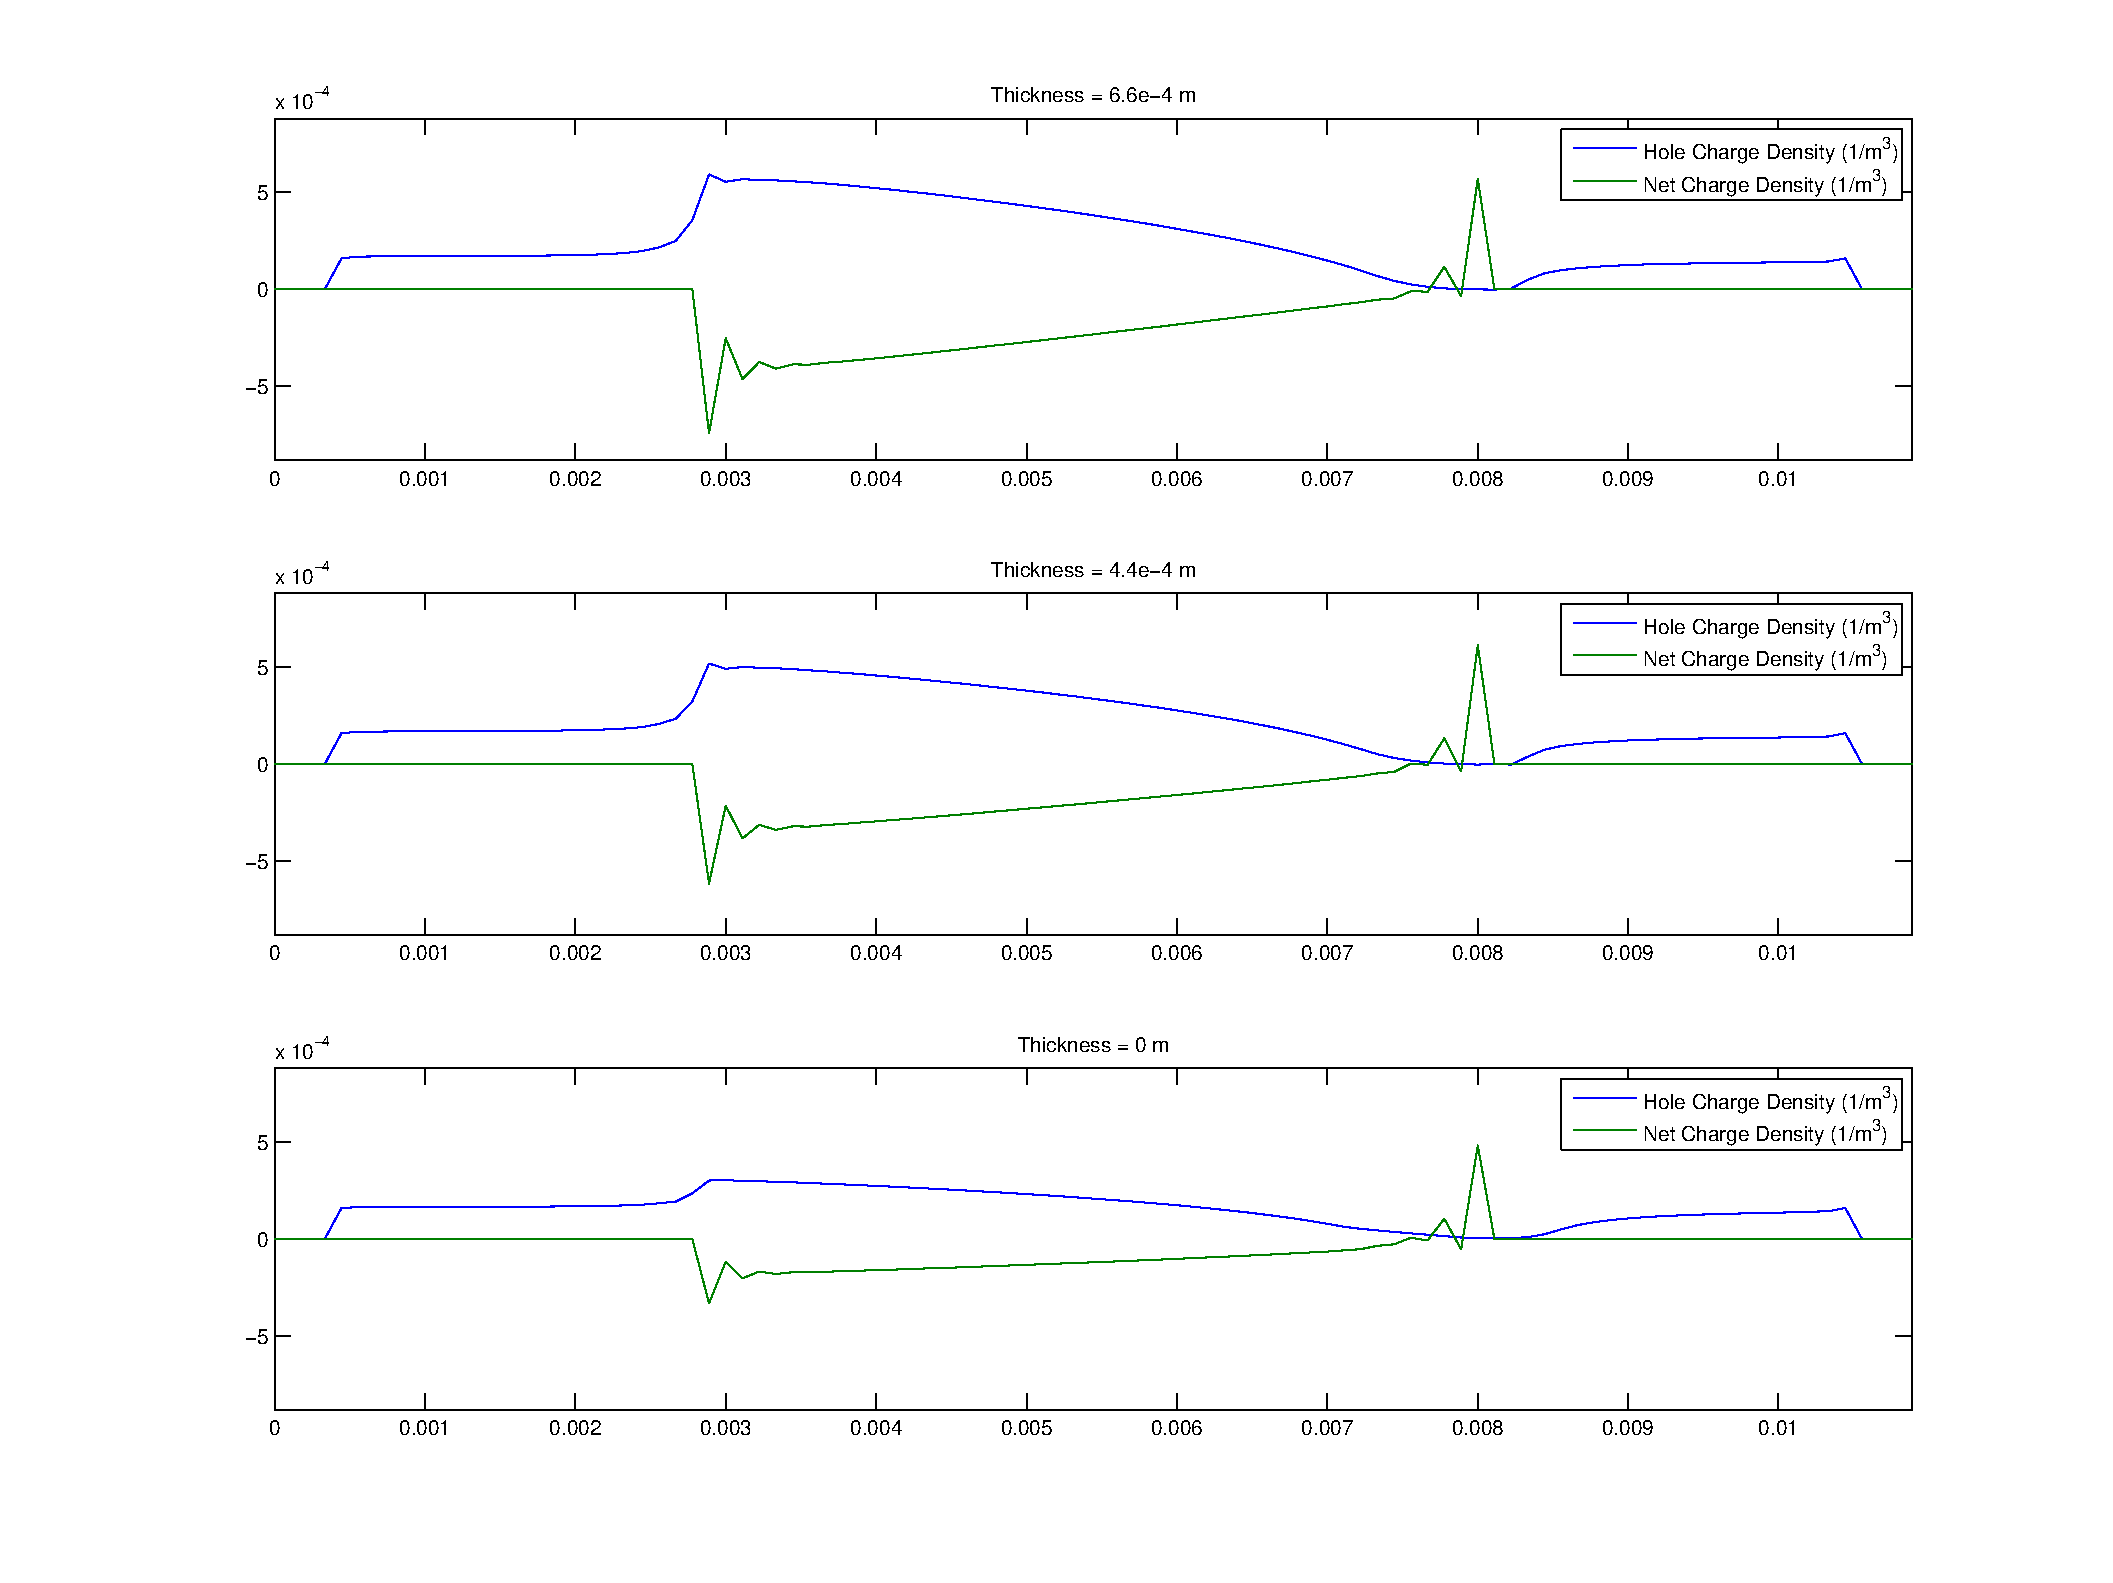
\includegraphics[scale=0.40]{2D_Memristor_netq_hole}
\caption{} 
\label{thick_netq_p}
\end{figure}

As shown in the previous chapter, the electric field has the highest value where lithium ions accumulate. The figure \ref{thick_efield} shows the change in the shape of the electric field as PEDOT:PSS gets thinner. For all thicknesses most of the potential drop occurs where lithium ions accumulate and it is concentrated at the surface of the PEDOT:PSS. 

Above plots showed that changing the thickness of the PEDOT:PSS does not have a drastic effect in the operation of the memristor since most of the changes occur at the interface between electrolyte and PEDOT:PSS. 1-D approximation of the polymer conductor contains all the necessary physics for the simulation of the memristor described in chapter 5.

\begin{figure}[!htp]
\centering
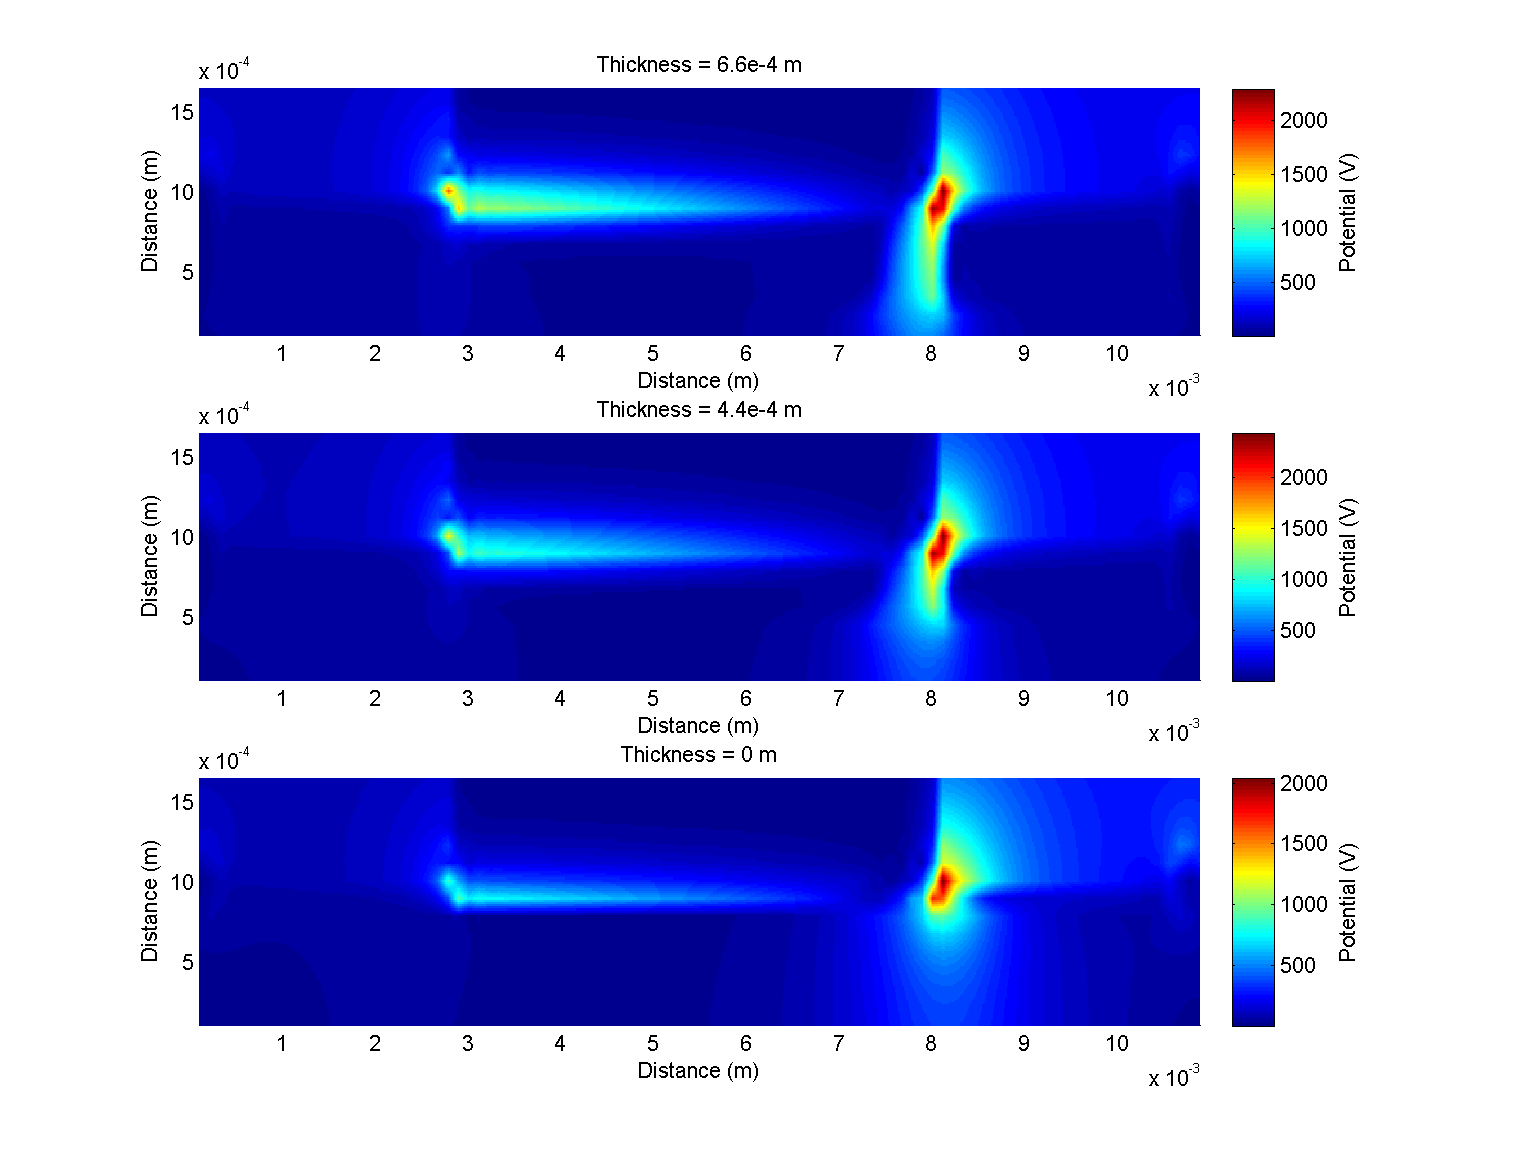
\includegraphics[scale=0.50]{2D_Memristor_Thick_E}
\caption{} 
\label{thick_efield}
\end{figure}


\clearpage
\section{2-D Memristor Simulation Using a Potential Pulse Train}

Following results are generated using the boundary and initial conditions from section 5.4.1 in order to show the differences between 1-D and 2-D memristor models. Even though the general trend of the normalized resistance is similar for plots (\ref{MemResTrain} and \ref{2D_mem_train}), there are two essential differences. The movement of the lithium ions controls the change in the resistivity over time therefore the response time of the device is dependent on the speed of the lithium ions which is a function of mobility and the electric field. In 1-D simulations the vertical mobility of the lithium needs to be adjusted in order to account for the thickness of the electrolyte. Because of this the mobility of the lithium has different values in different directions. Different resistivity measurements for different metal contacts indicate that the lithium ions moved into the PEDOT:PSS relatively fast and holes were not able to keep up with this change. 
      
\begin{figure}[!htp]
\centering
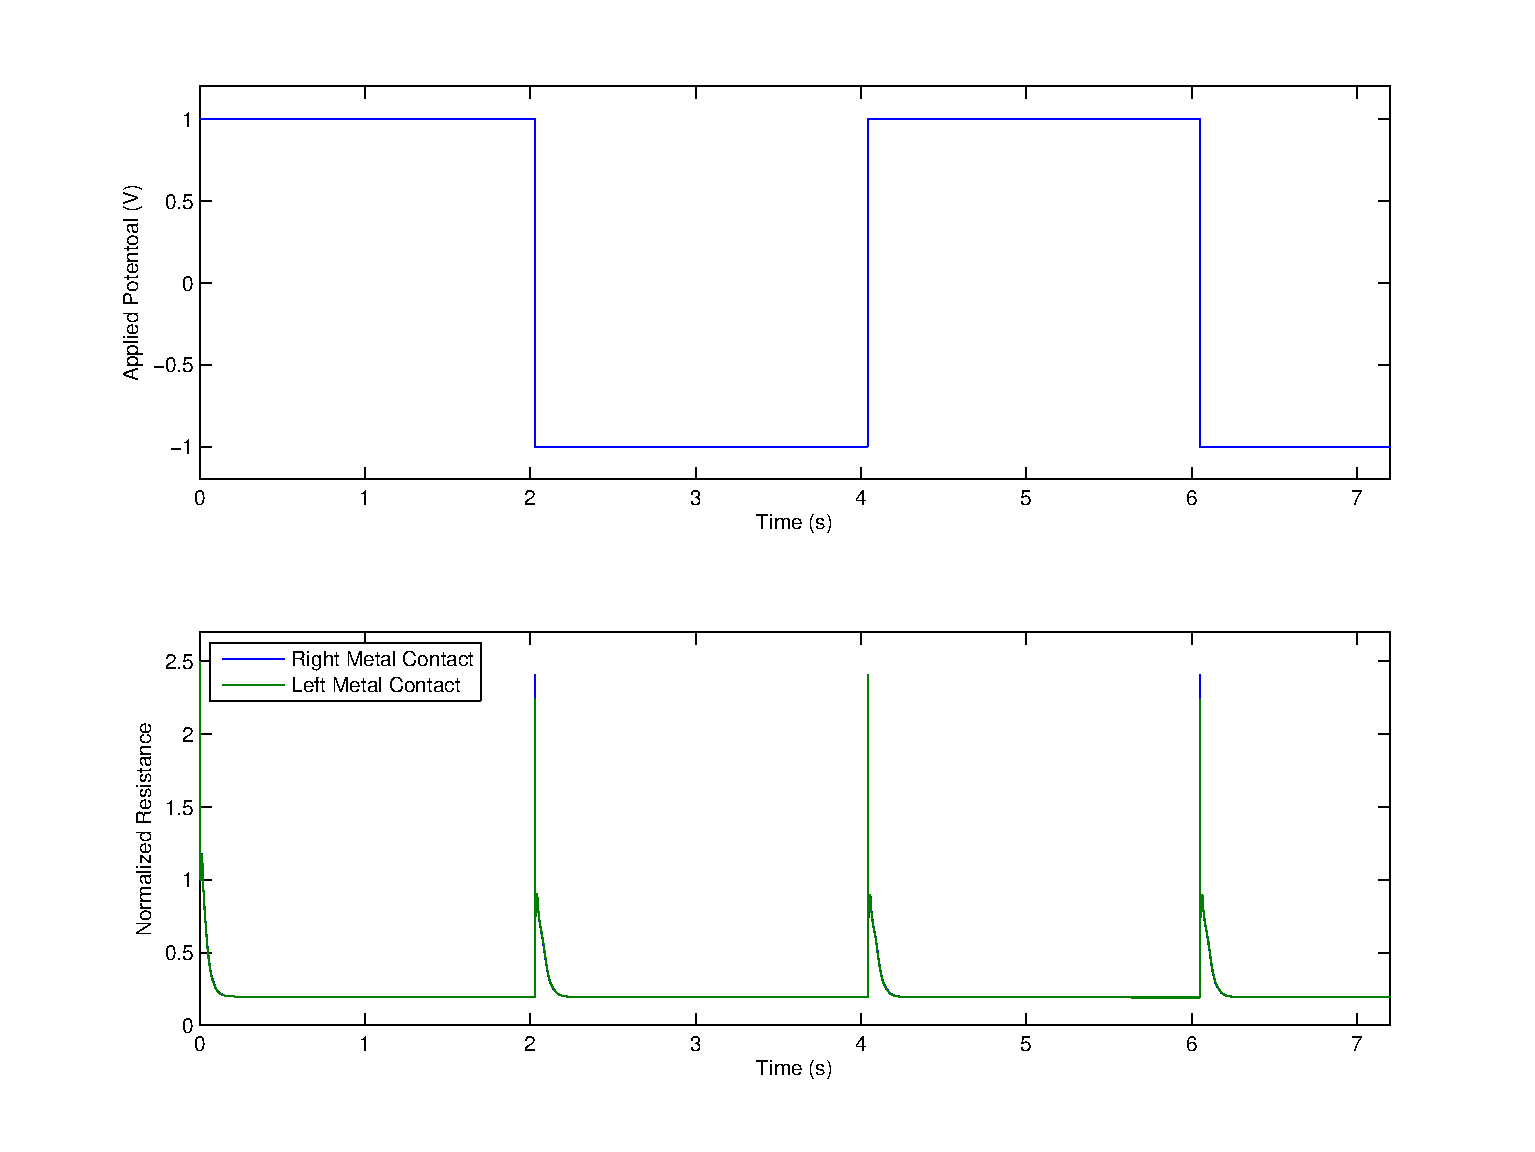
\includegraphics[scale=0.50]{2D_Memristor_Pulse_Train}
\caption{Applied potential and normalized resistance over time of a 2-D memristor} 
\label{2D_mem_train}
\end{figure}


\begin{figure}[!htp]
\centering
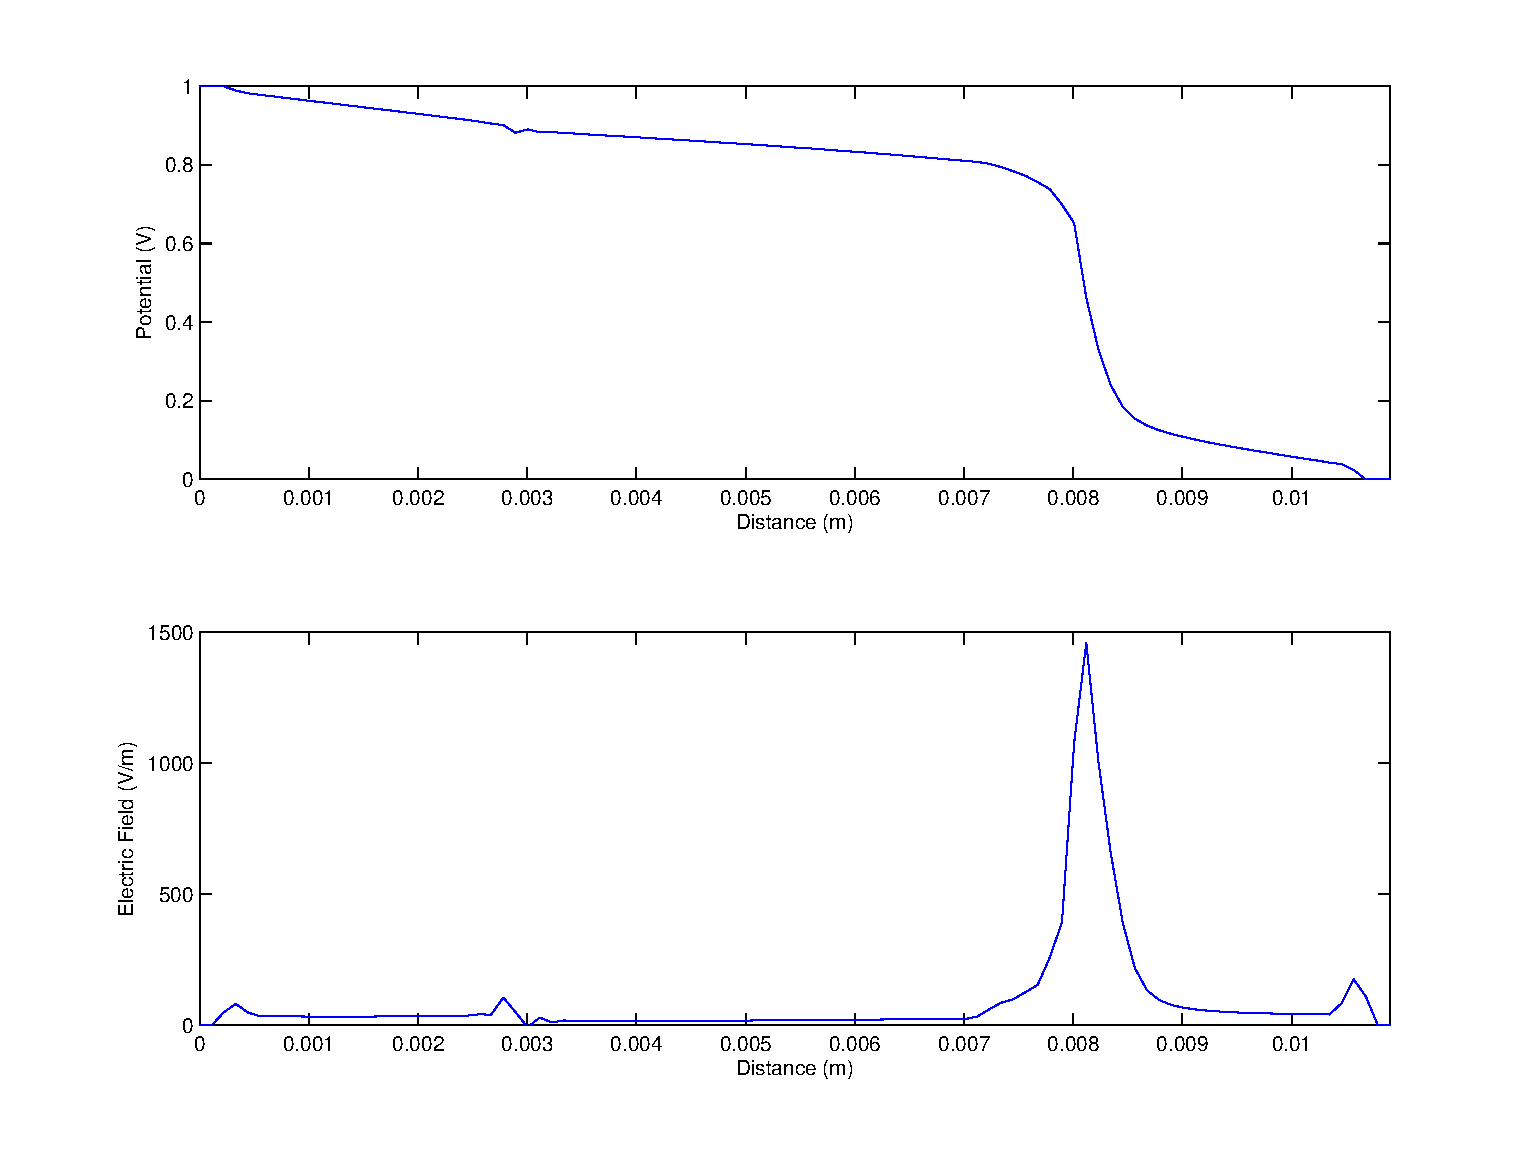
\includegraphics[scale=0.50]{2D_Memristor_Pulse_Train_EV}
\caption{} 
\label{}
\end{figure}

\begin{figure}[!htp]
\centering
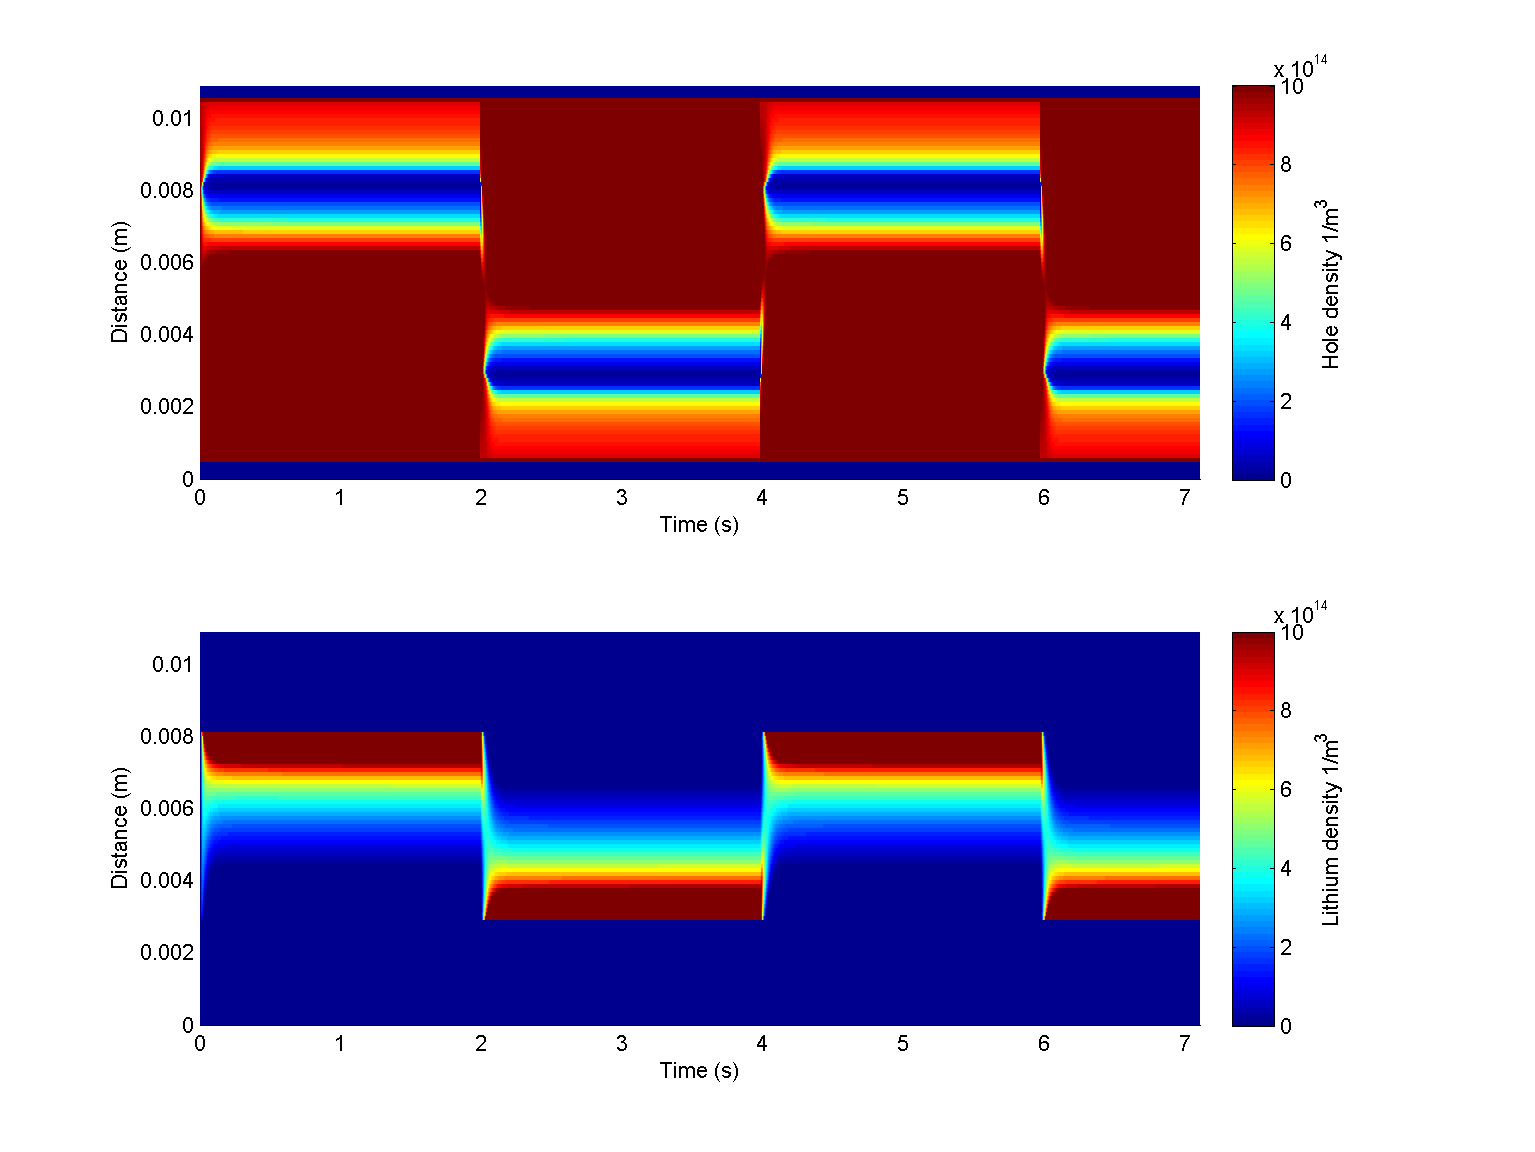
\includegraphics[scale=0.50]{2D_Memristor_Pulse_Lithium_Hole}
\caption{} 
\label{}
\end{figure}

\begin{figure}[!htp]
\centering
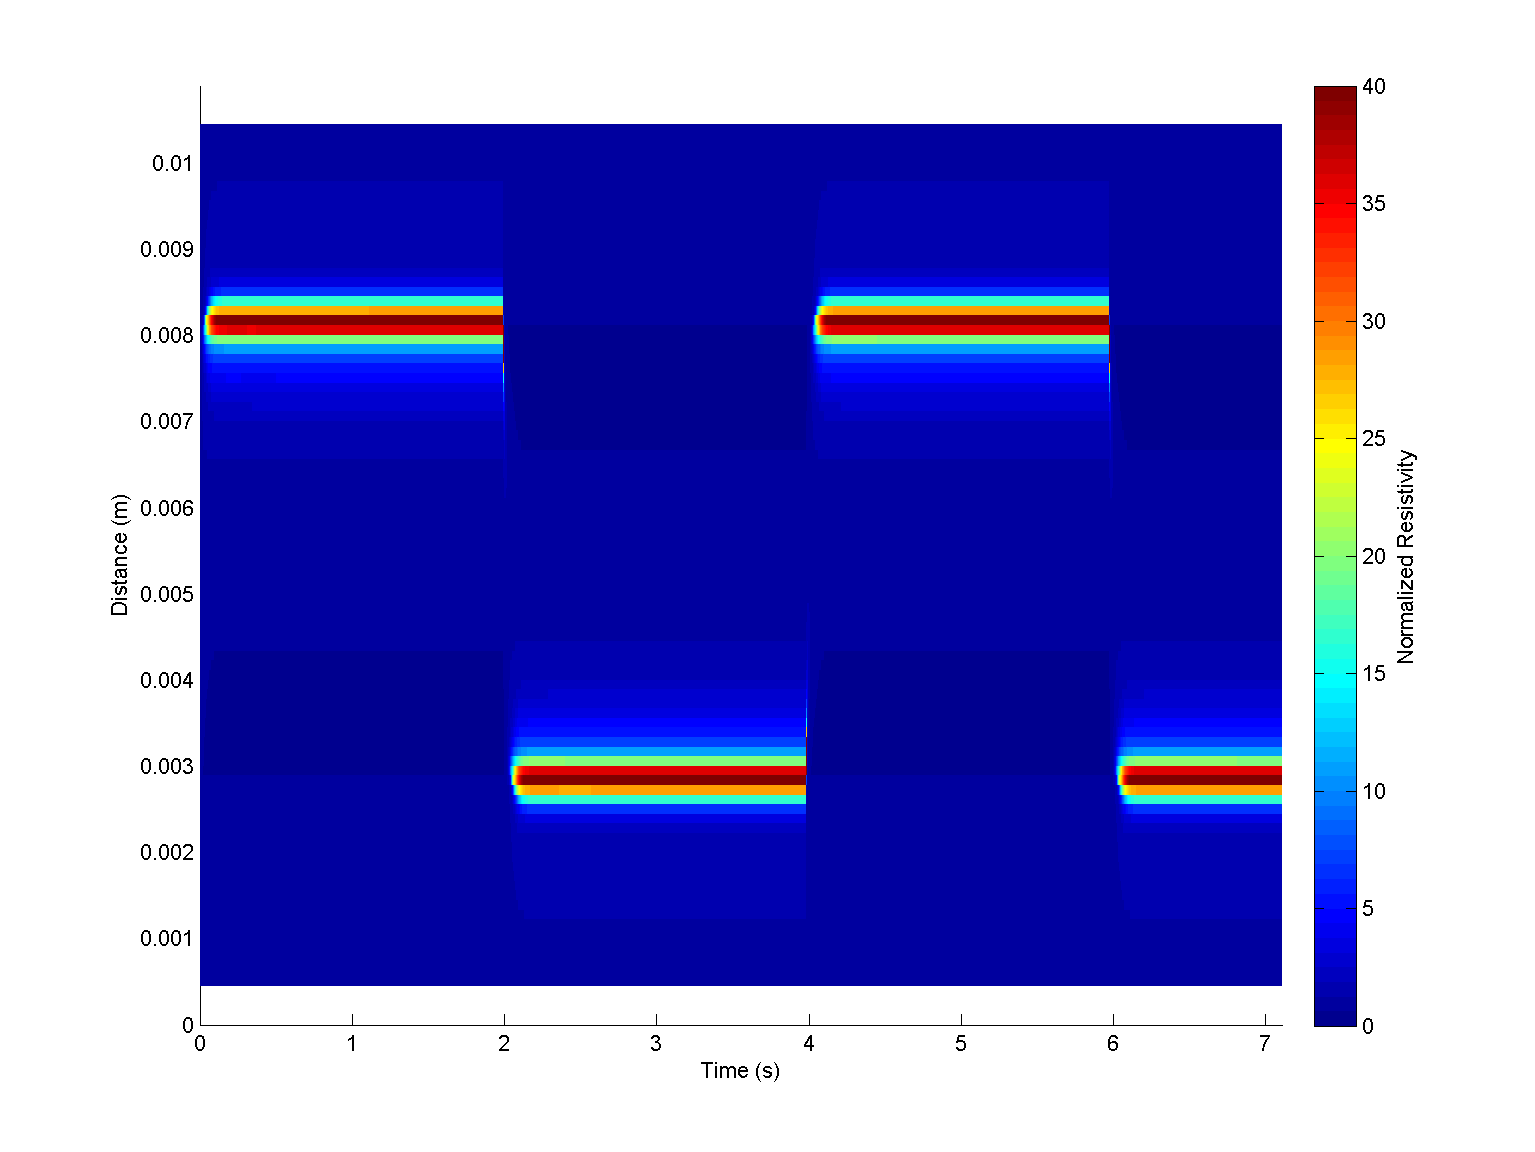
\includegraphics[scale=0.50]{2D_Memristor_Resistivity}
\caption{} 
\label{}
\end{figure}



\begin{figure}[!htp]
\centering
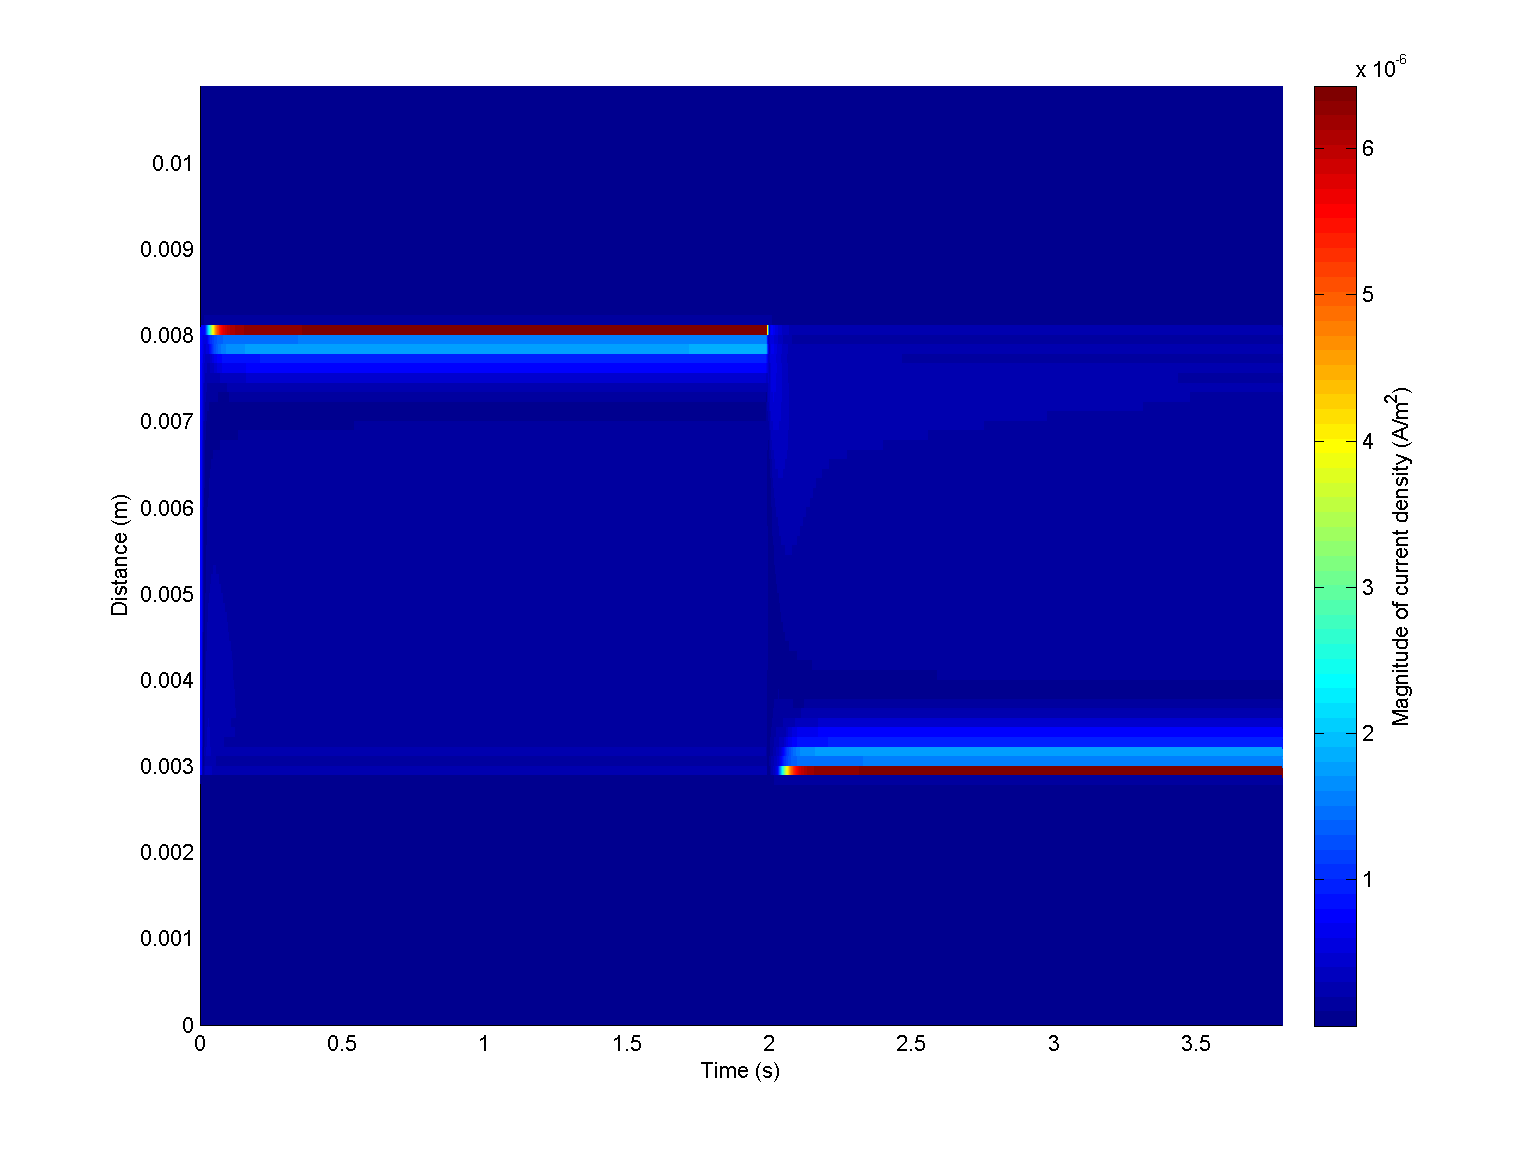
\includegraphics[scale=0.50]{2D_Memristor_Pulse_Lithium_J}
\caption{} 
\label{}
\end{figure}


\clearpage
\section{2-D Memristor Simulation Using a Sinusoid}

\begin{figure}[!htp]
\centering
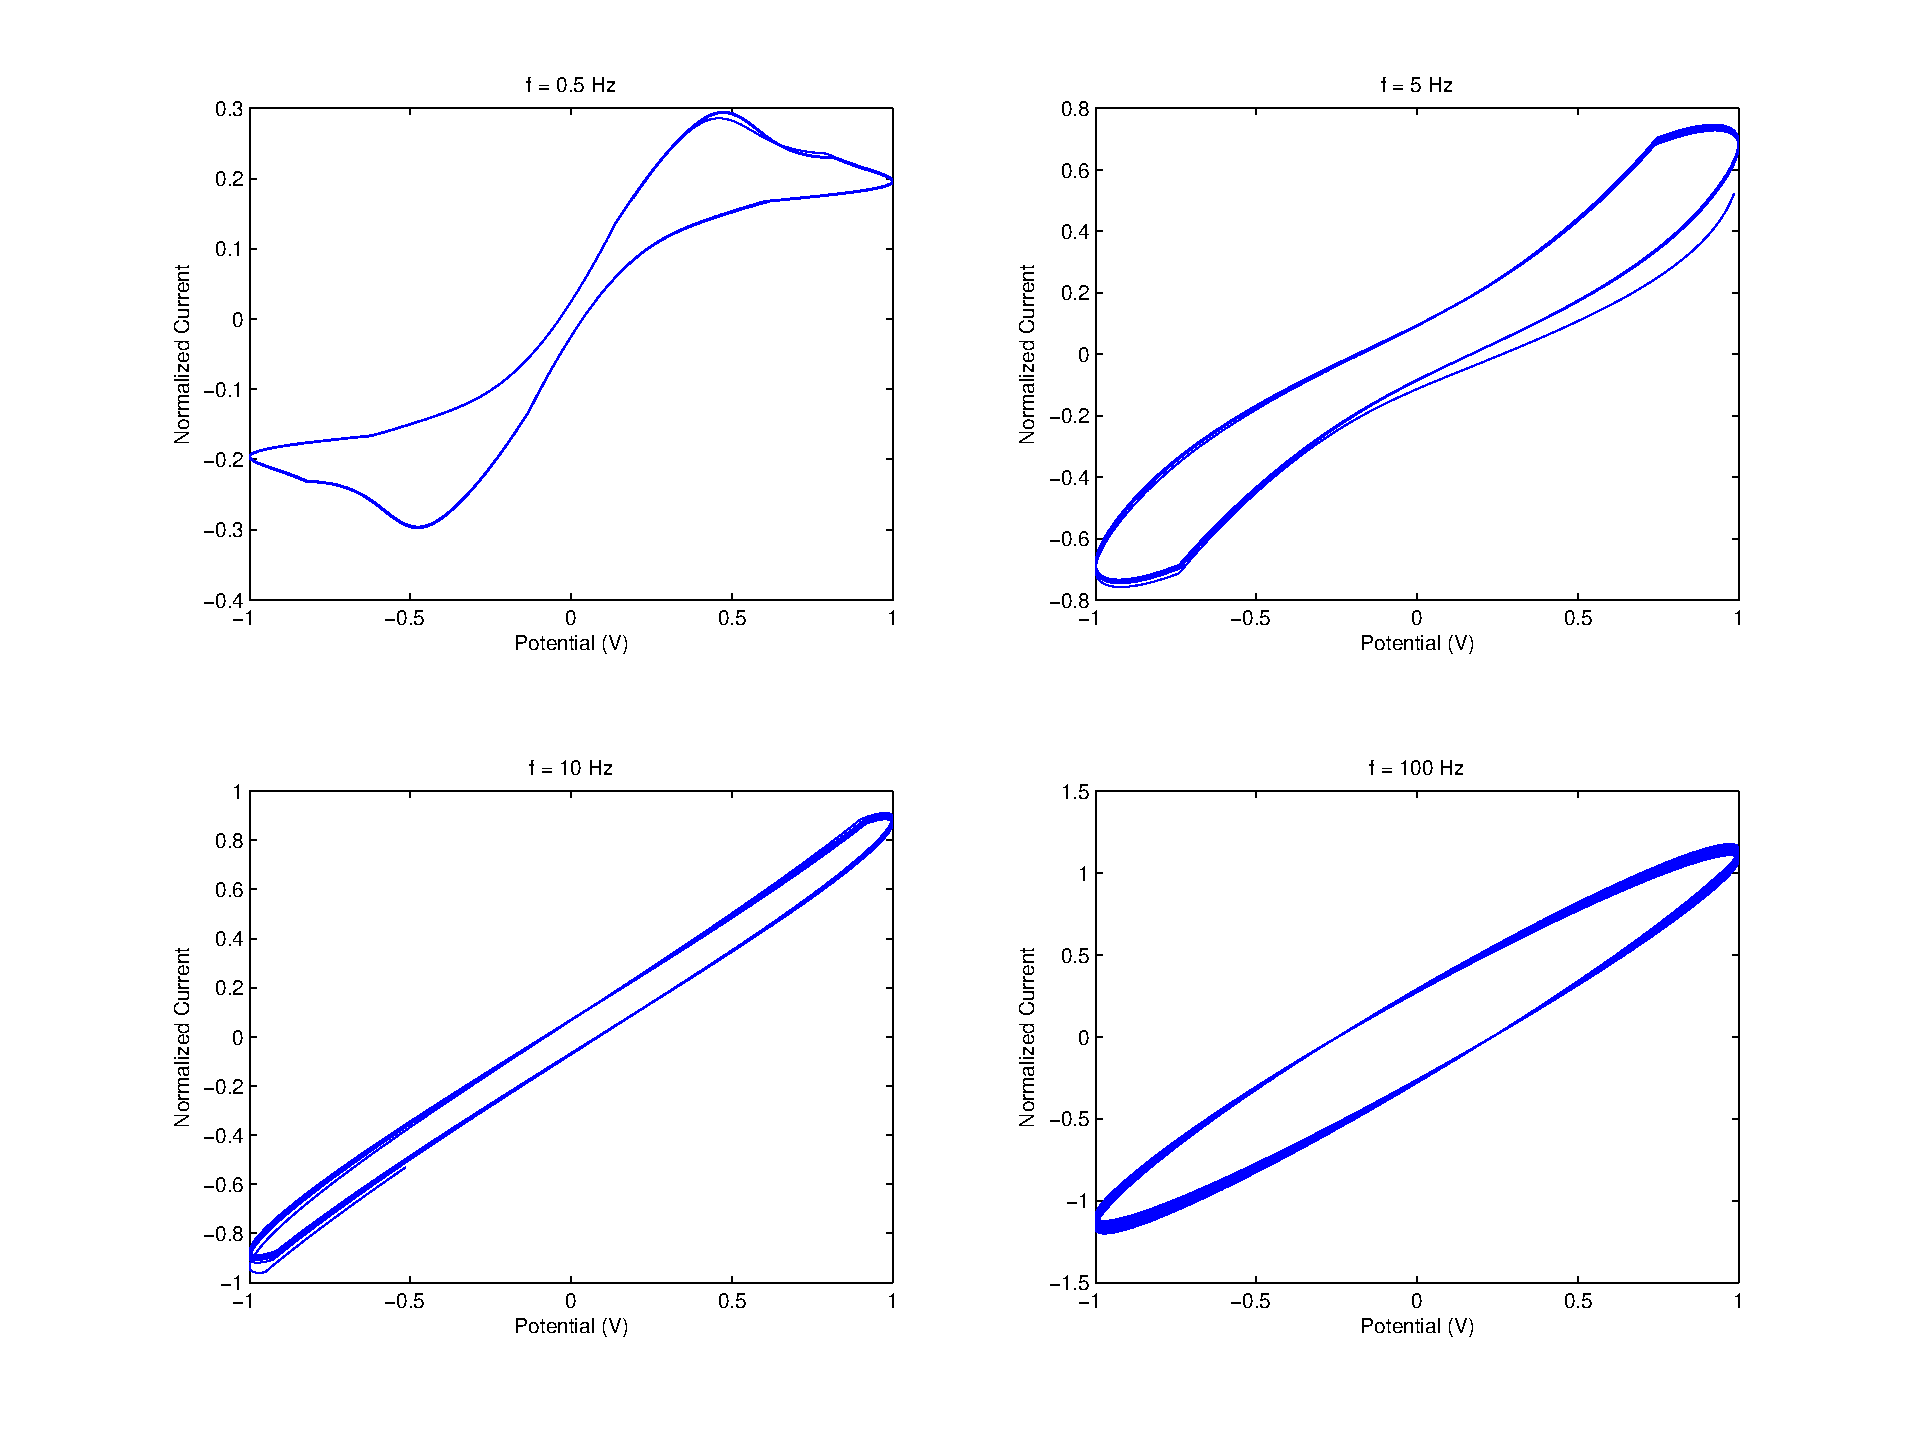
\includegraphics[scale=0.45]{2D_Memristor_bowtie_f}
\caption{} 
\label{}
\end{figure}


\begin{figure}[!htp]
\centering
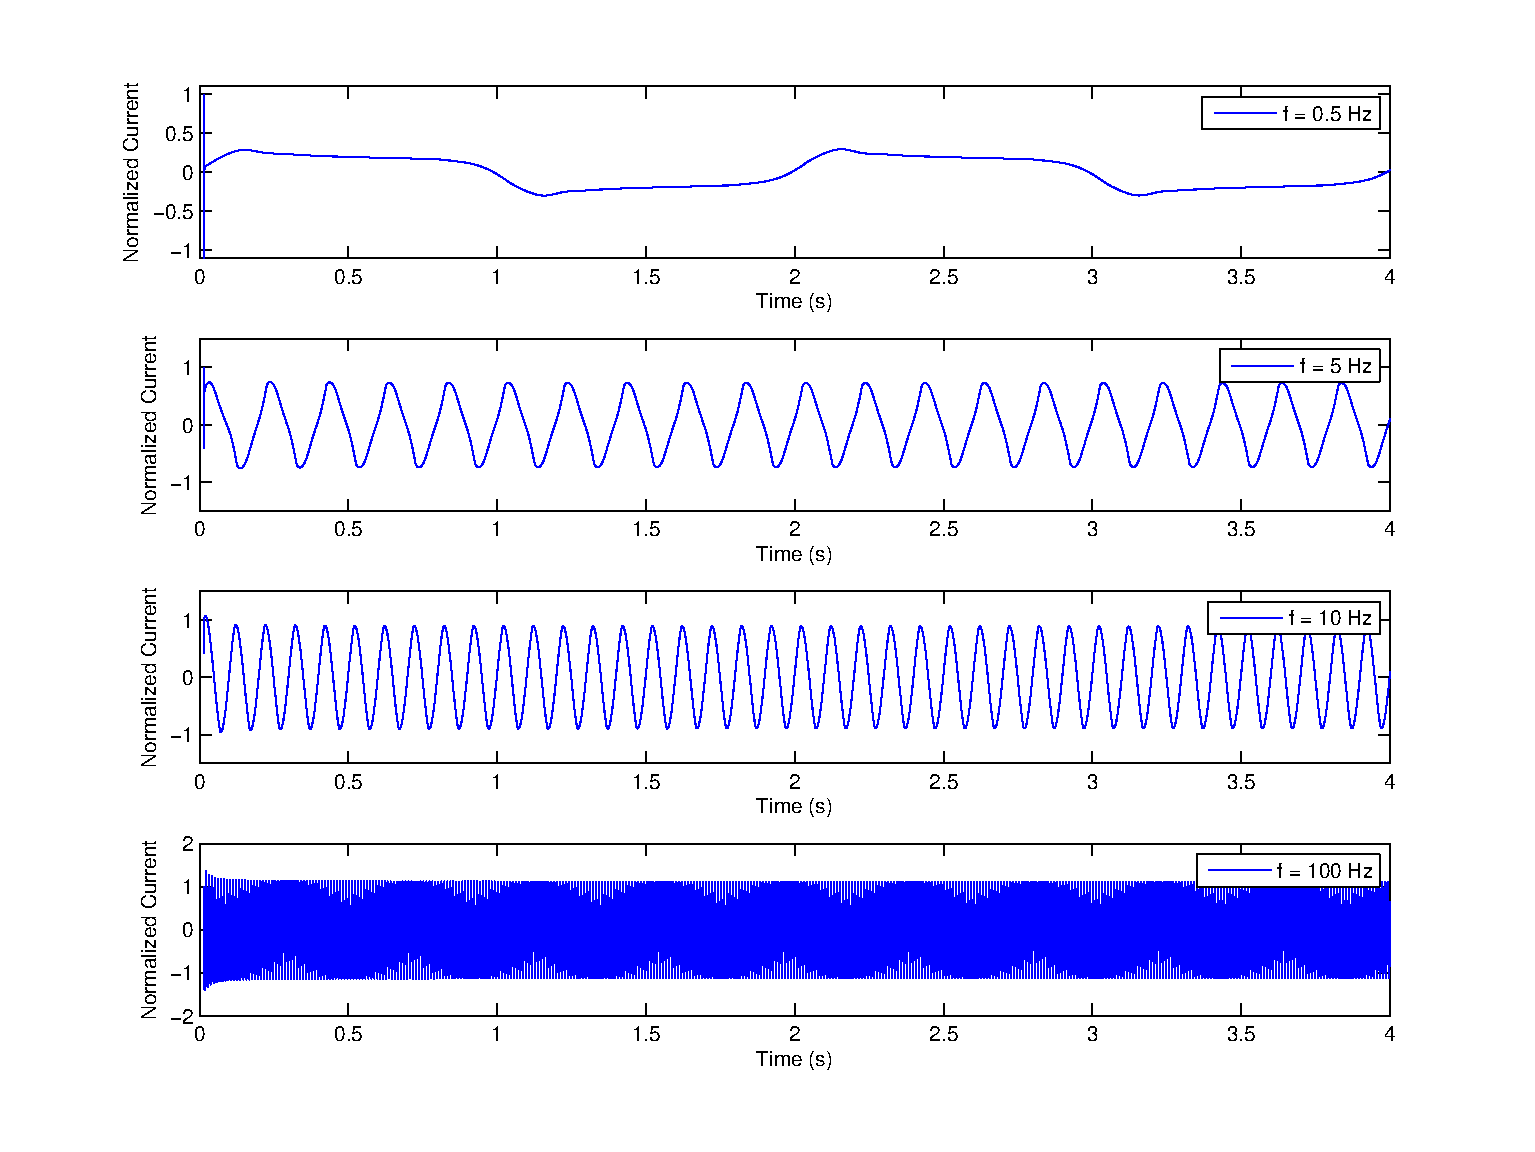
\includegraphics[scale=0.50]{2D_Memristor_Current_f}
\caption{} 
\label{}
\end{figure}

\begin{figure}[!htp]
\centering
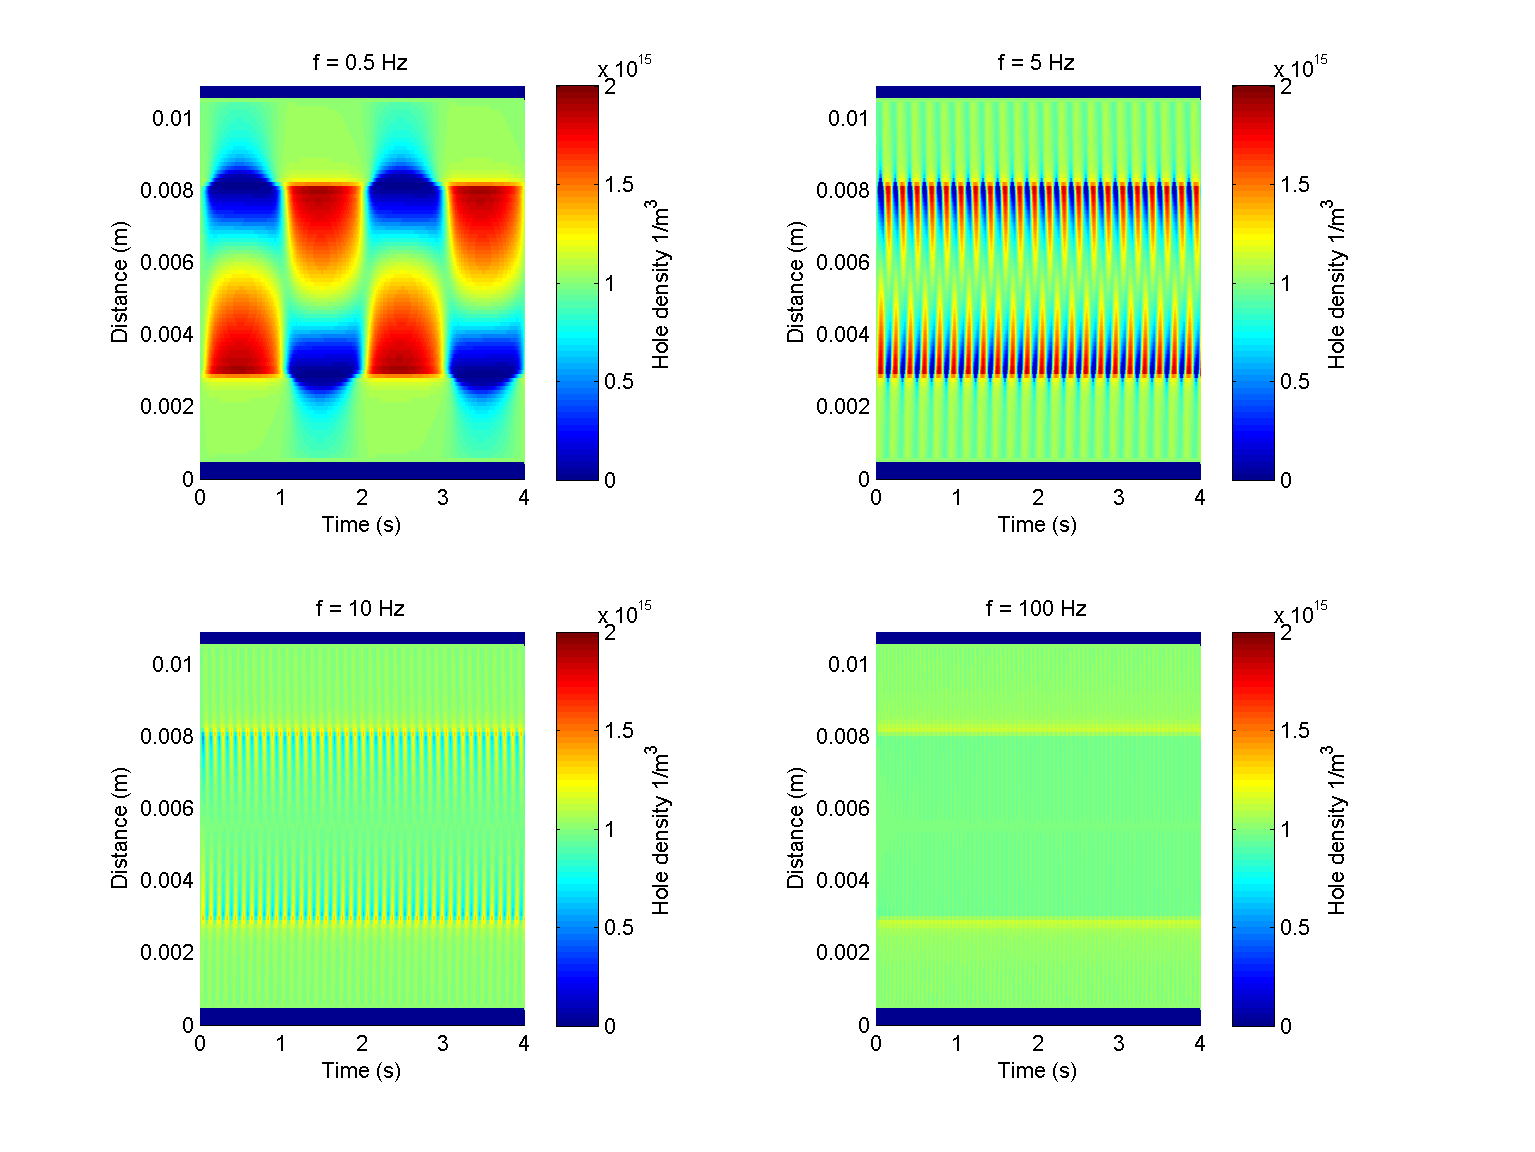
\includegraphics[scale=0.55]{2D_Memristor_f_Hole}
\caption{} 
\label{}
\end{figure}

\begin{figure}[!htp]
\centering
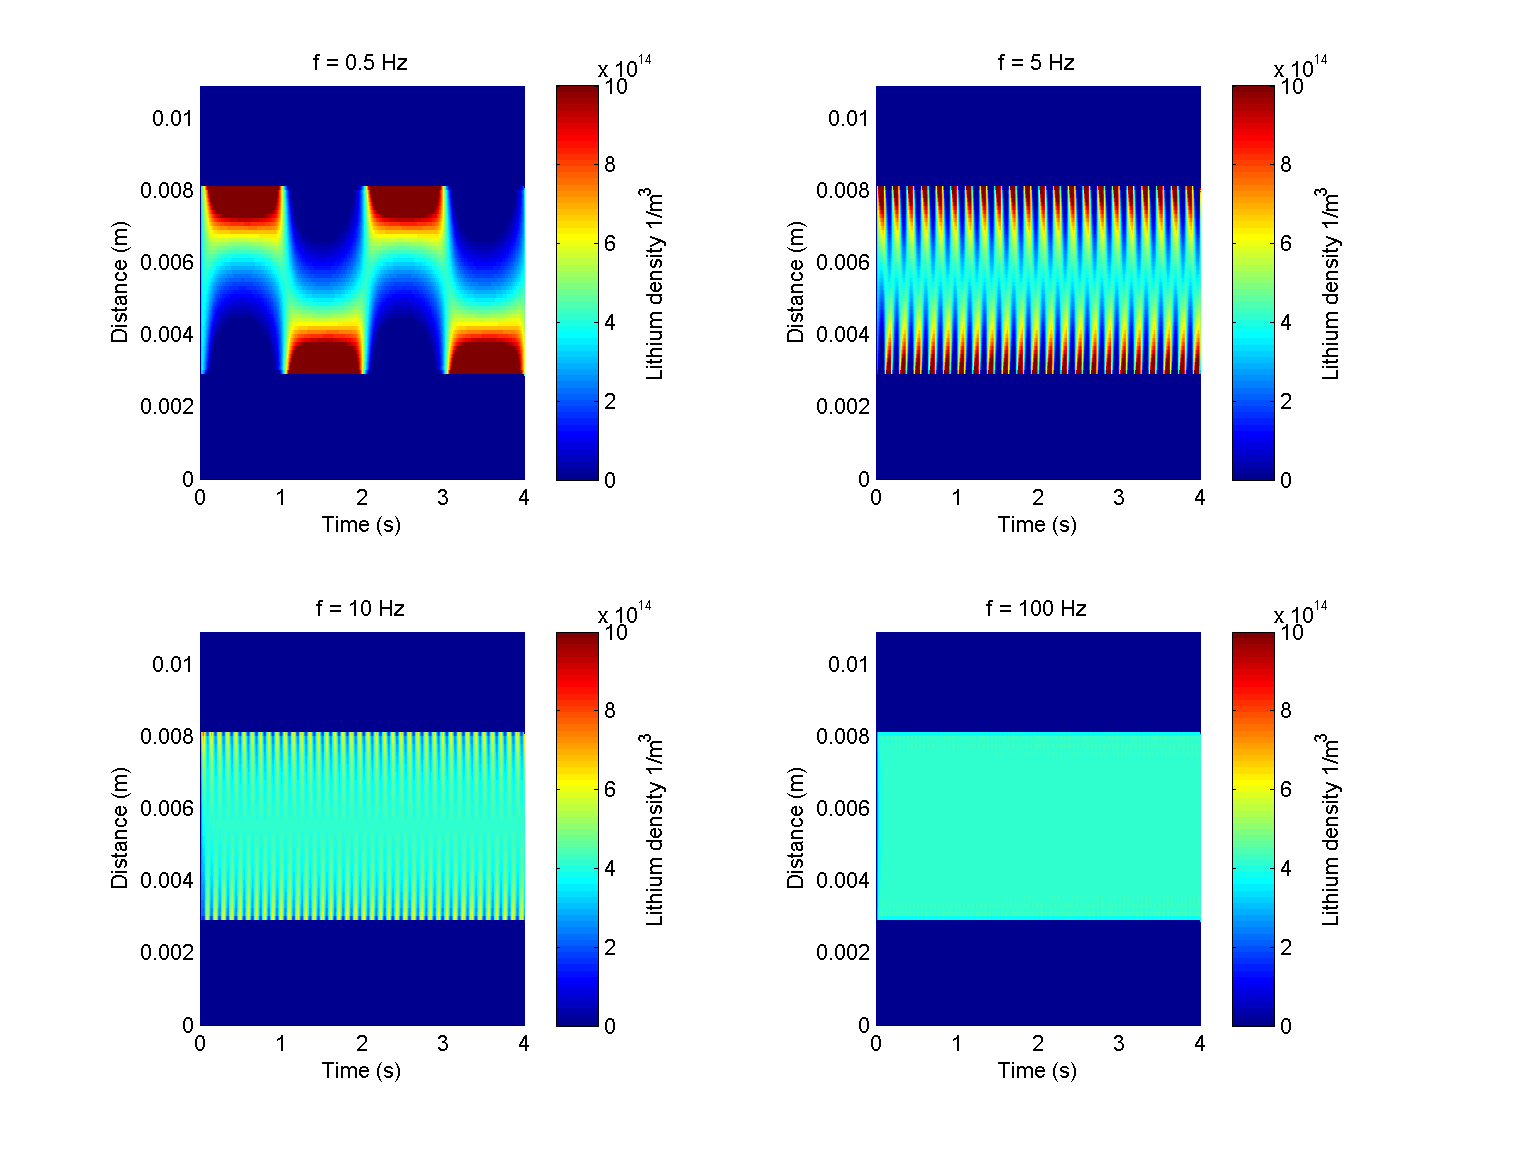
\includegraphics[scale=0.55]{2D_Memristor_f_Lithium}
\caption{} 
\label{}
\end{figure}

\begin{figure}[!htp]
\centering
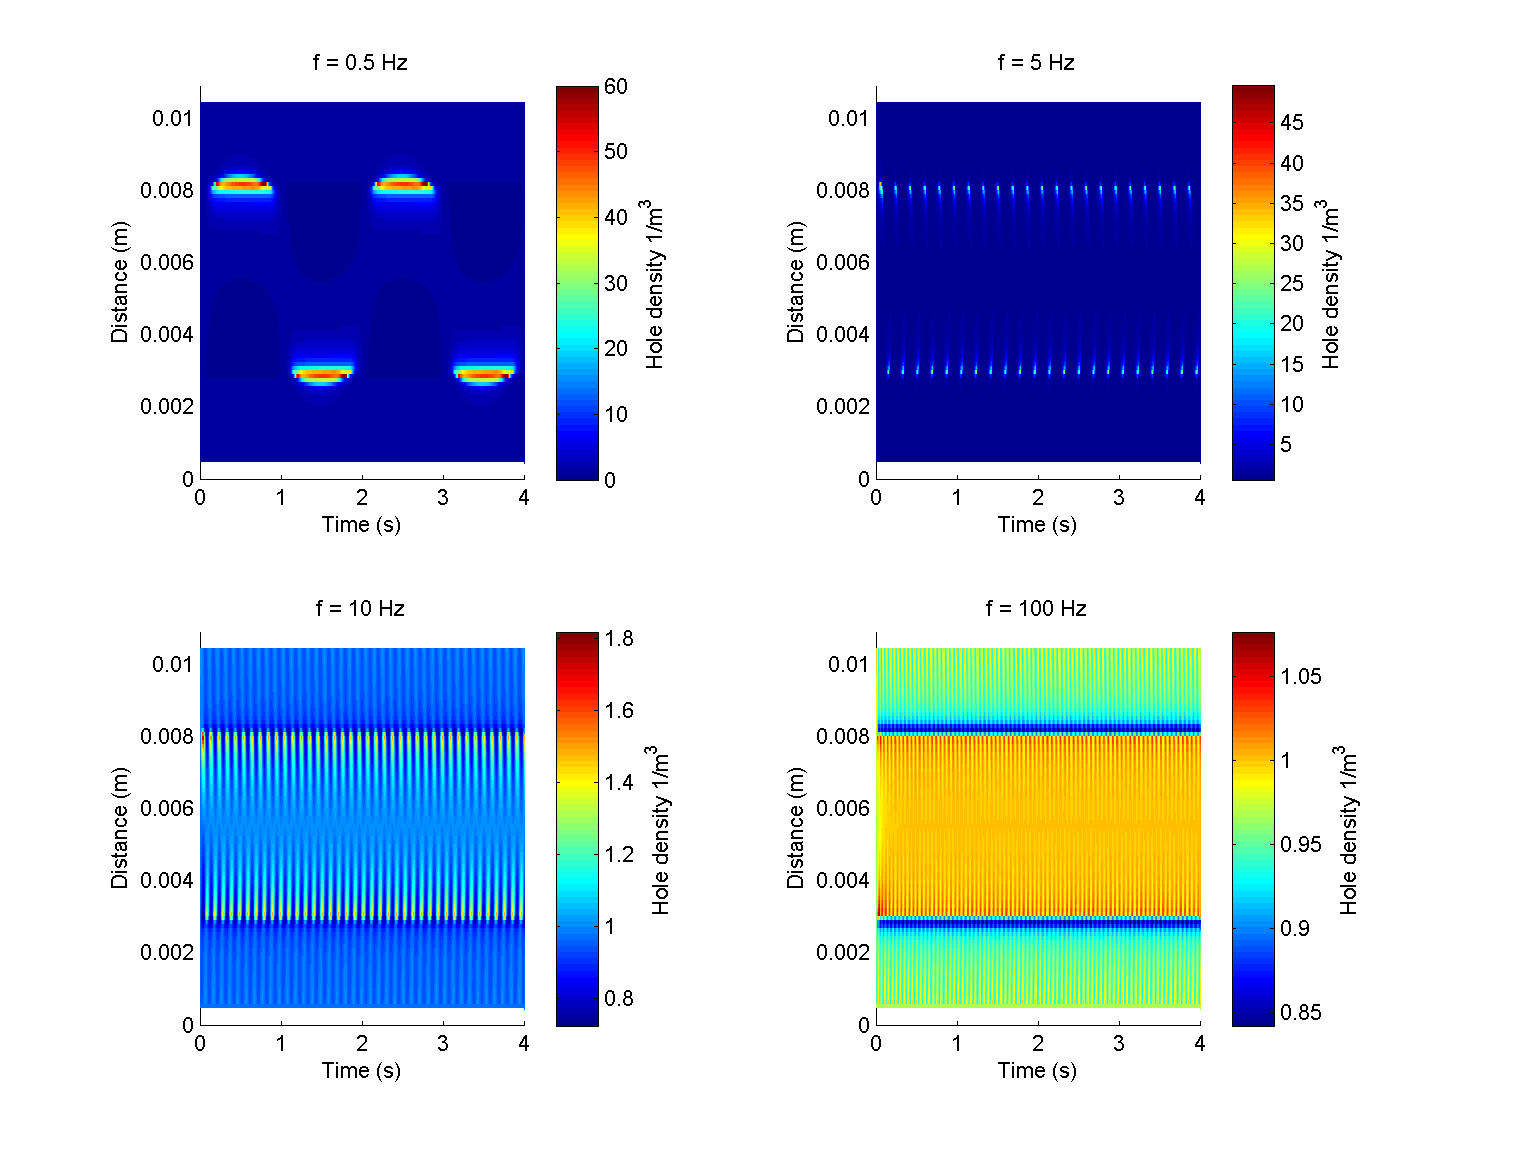
\includegraphics[scale=0.55]{2D_Memristor_f_Resistivity}
\caption{} 
\label{}
\end{figure}


\begin{figure}[!htp]
\centering
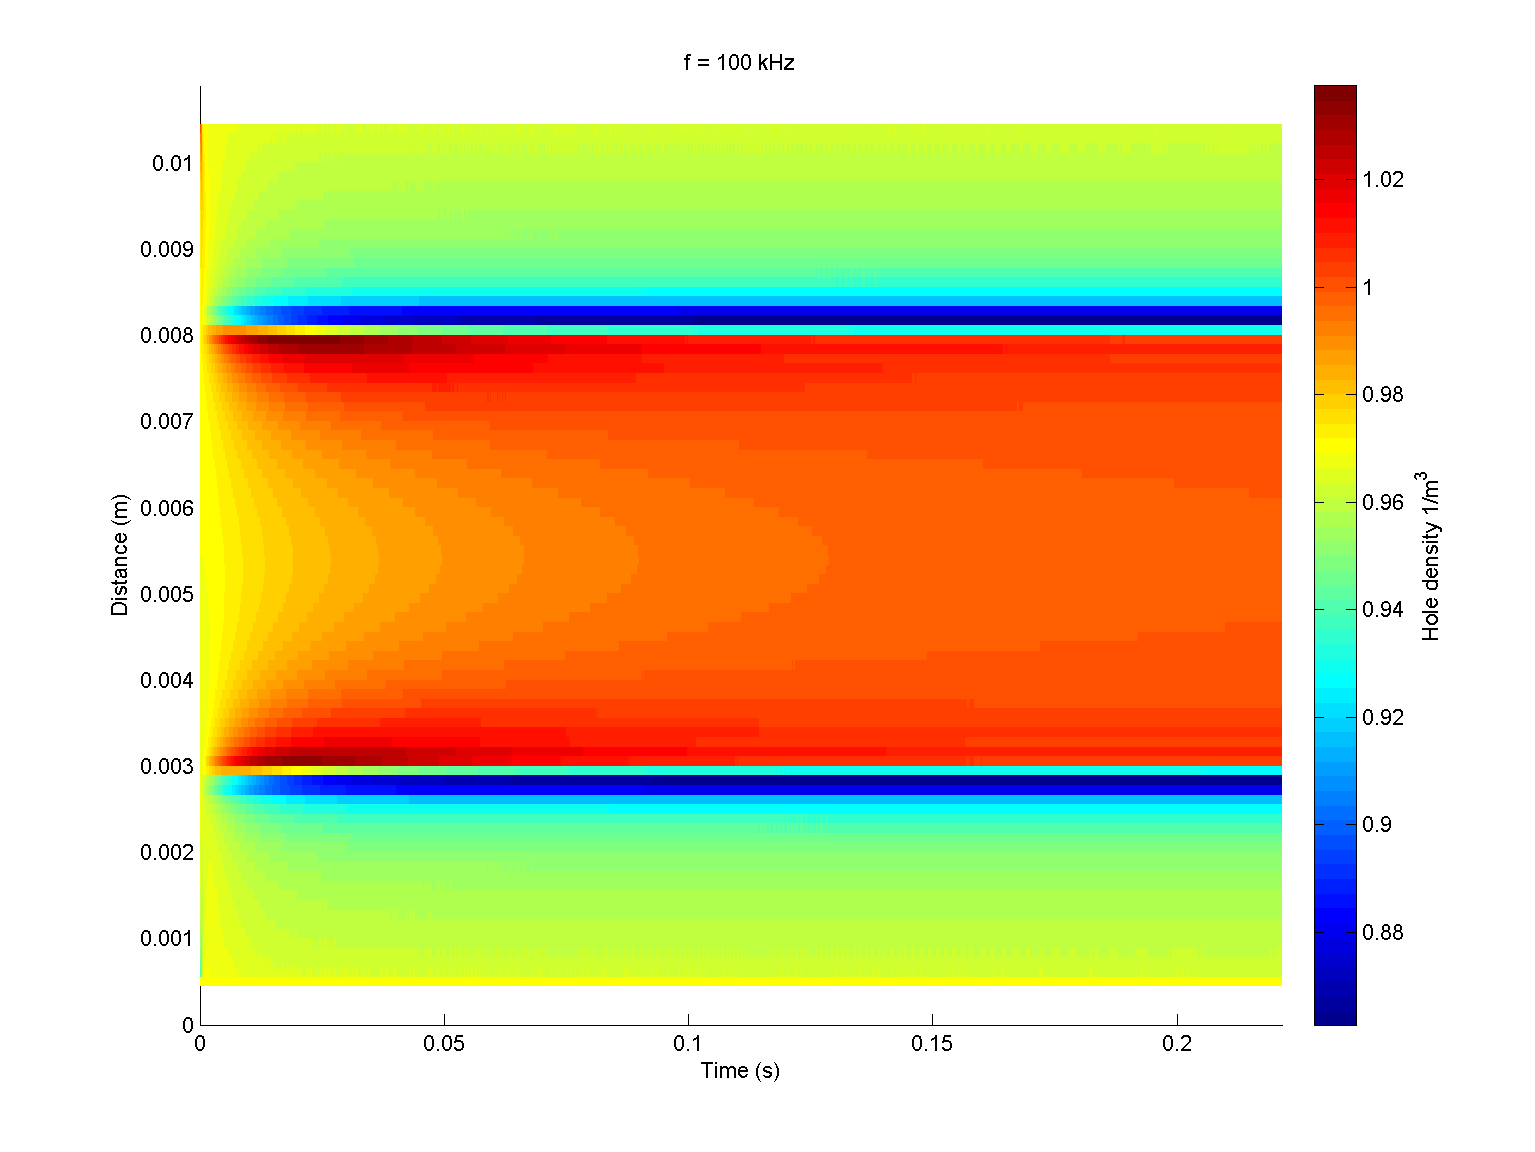
\includegraphics[scale=0.50]{2D_Memristor_f_Resistivity_1e5}
\caption{} 
\label{}
\end{figure}

\clearpage
\section{Experiment vs. Simulation}


\begin{figure}[!htp]
\centering
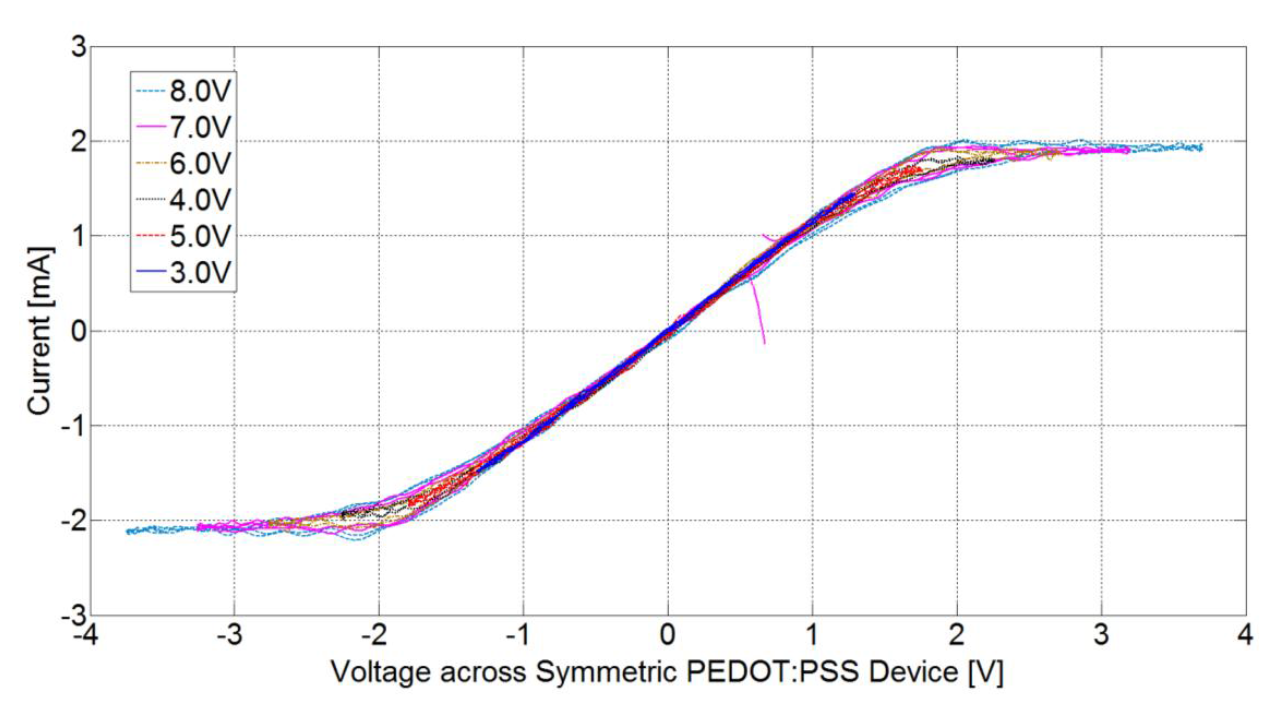
\includegraphics[scale=0.33]{memf1e-1}
\caption{} 
\label{}
\end{figure}


\begin{figure}[!htp]
\centering
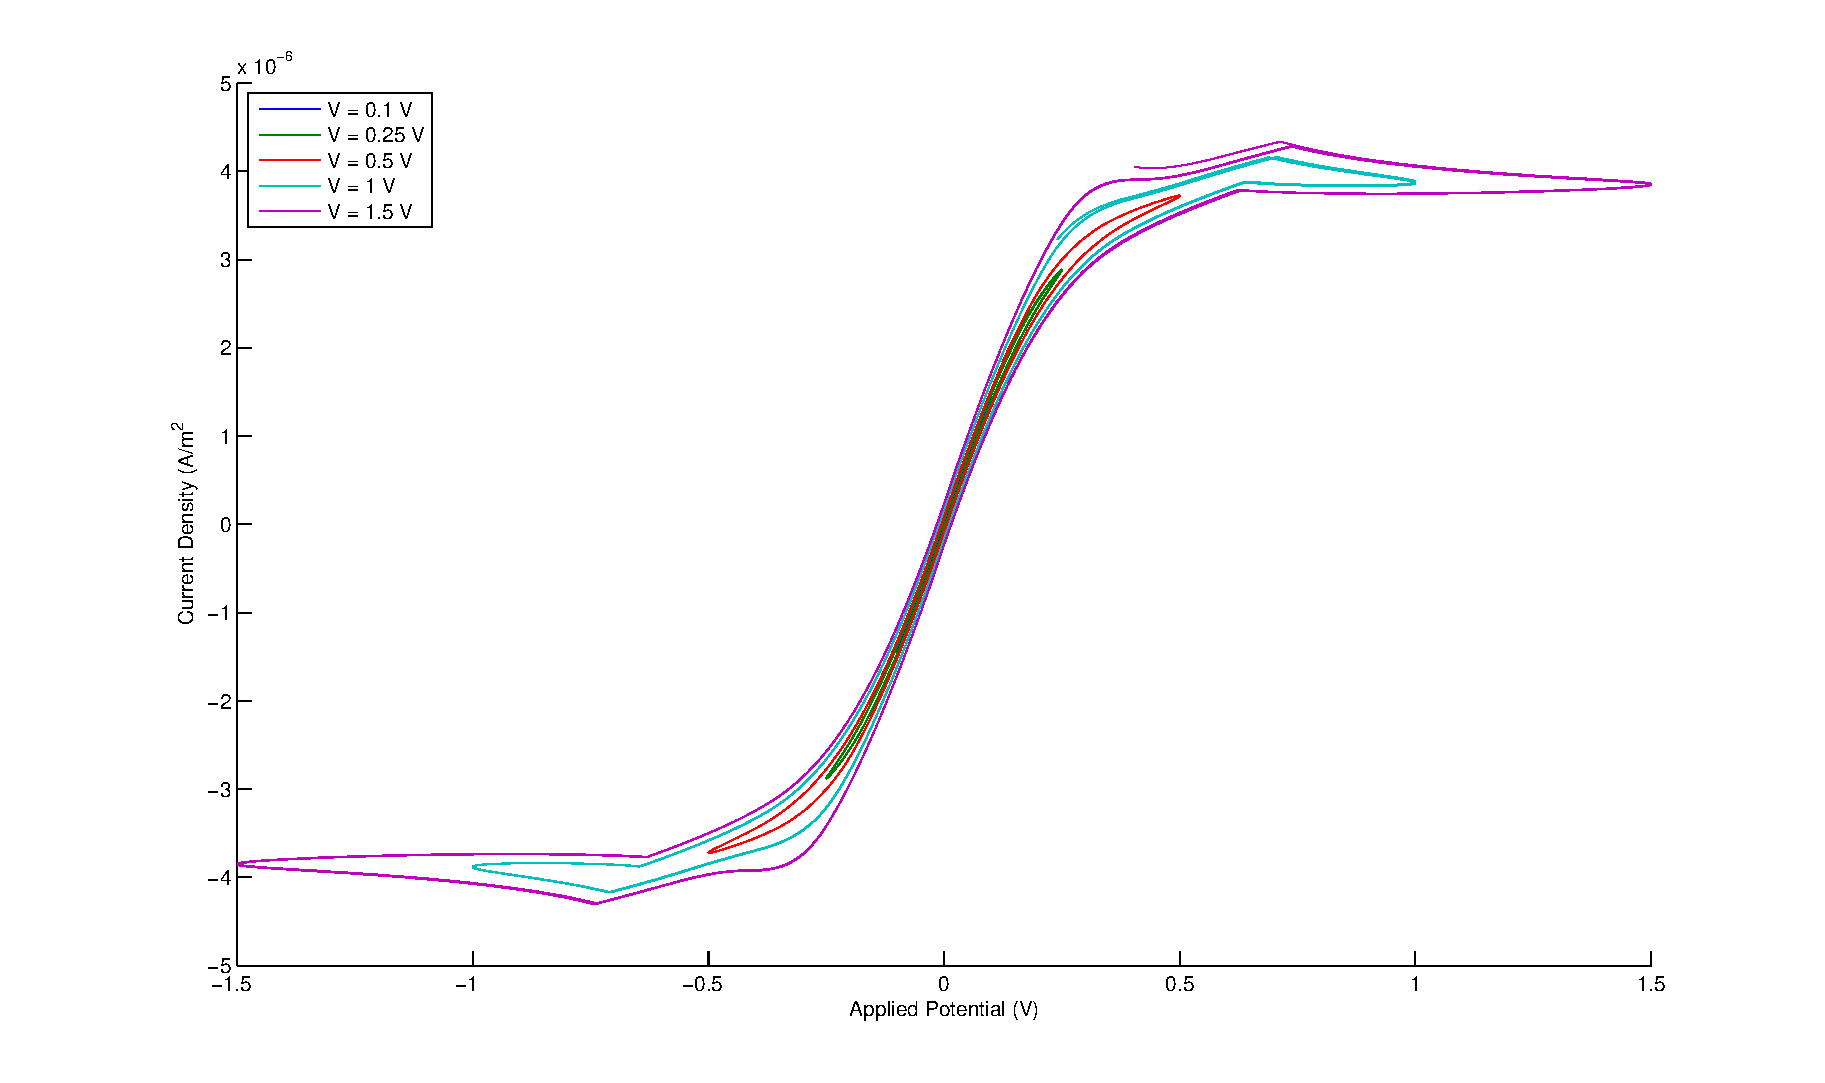
\includegraphics[scale=0.36]{Bowtief01Vchng}
\caption{} 
\label{}
\end{figure}

\clearpage

\begin{figure}[!htp]
\centering
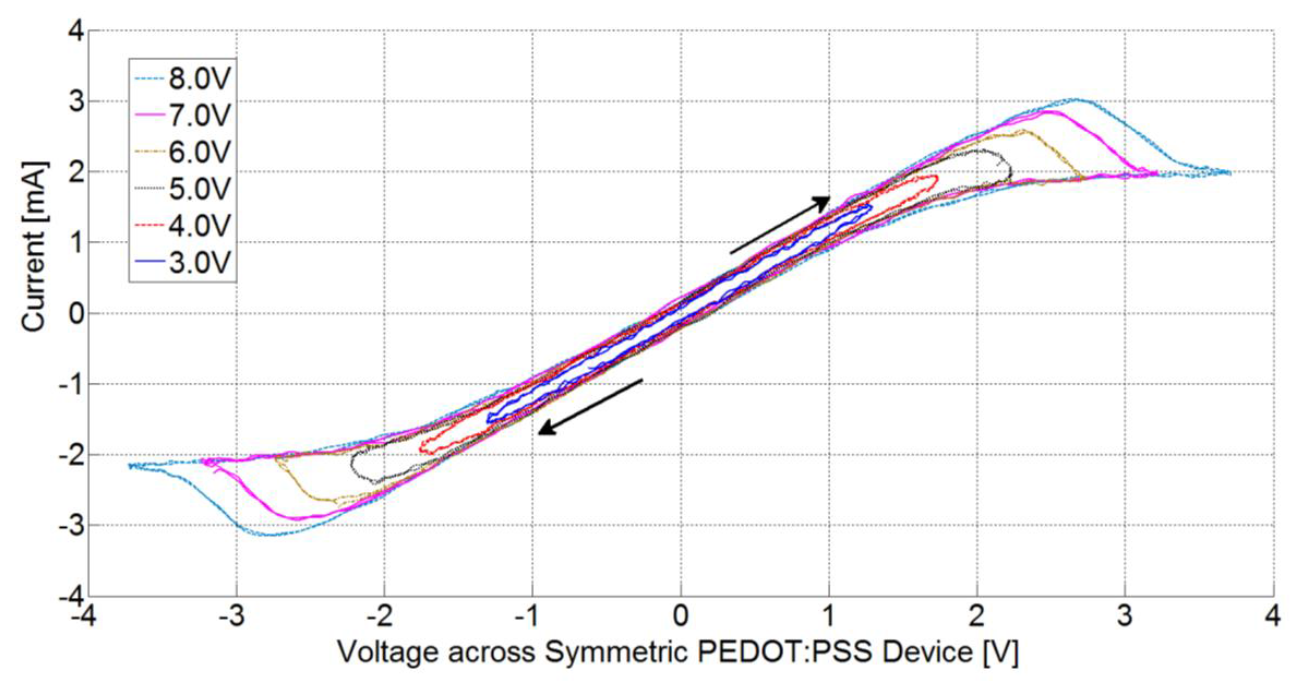
\includegraphics[scale=0.3]{memf1}
\caption{} 
\label{}
\end{figure}


\begin{figure}[!htp]
\centering
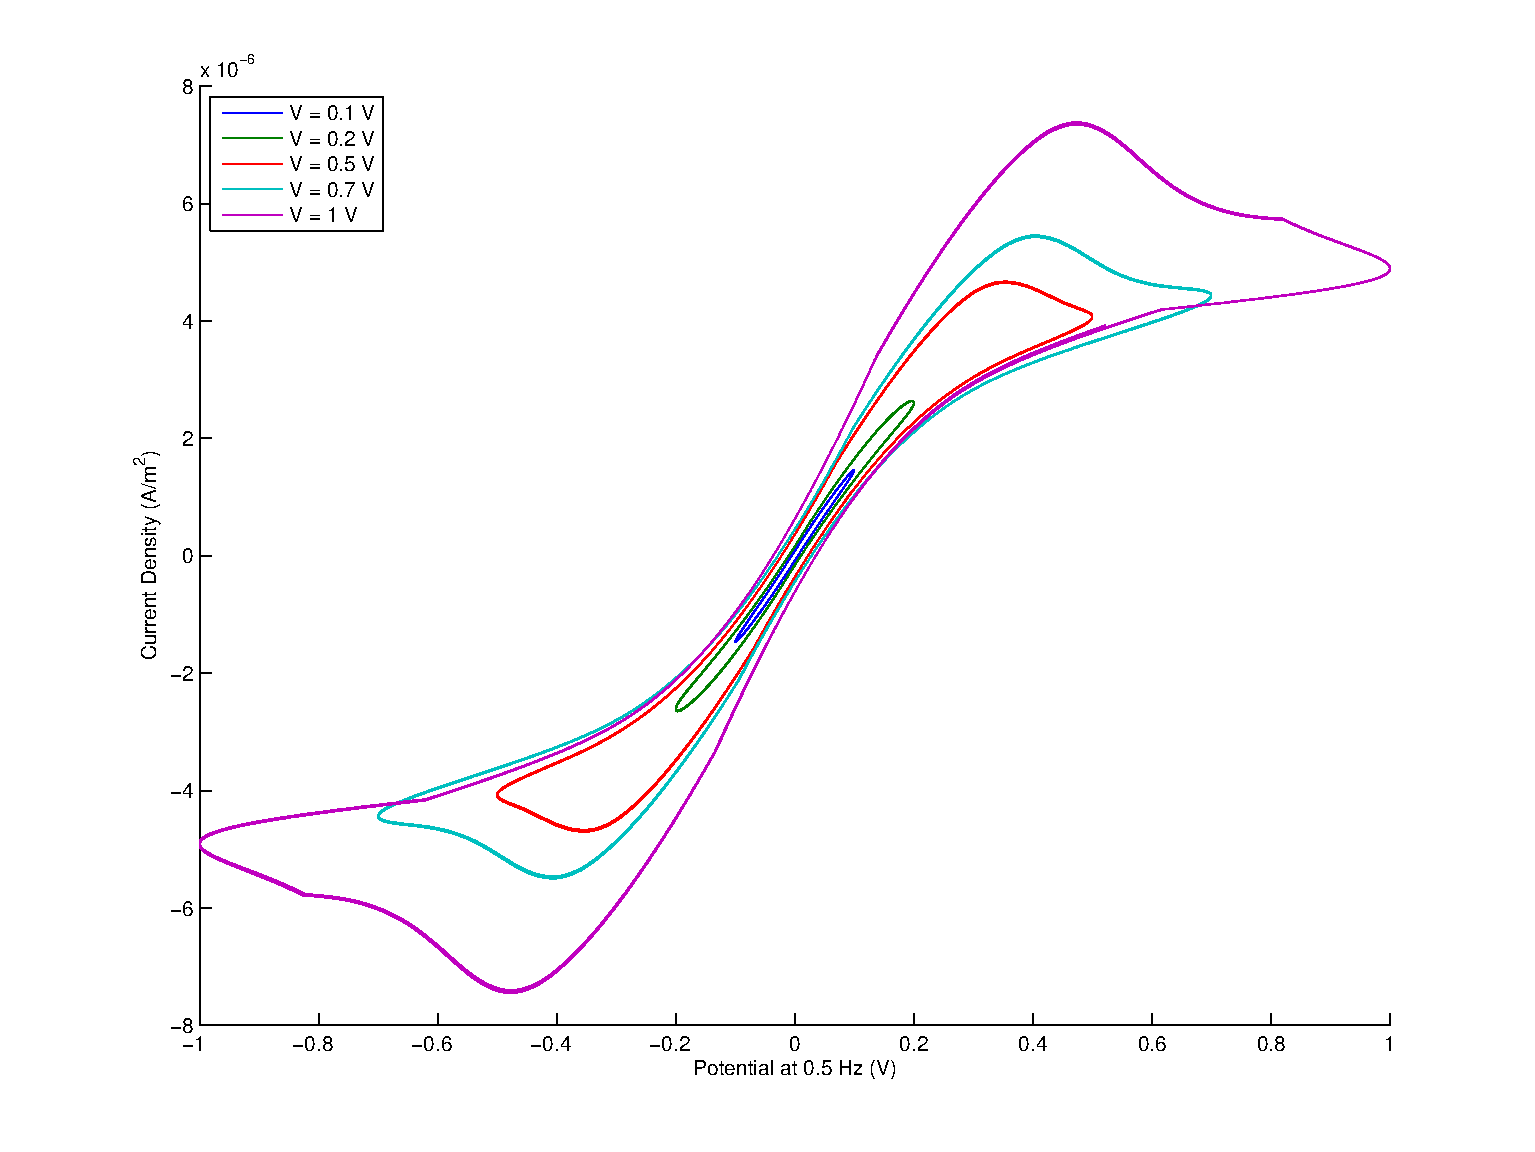
\includegraphics[scale=0.38]{2D_Memristor_5e-1Hz}
\caption{} 
\label{}
\end{figure}

\clearpage
\begin{figure}[!htp]
\centering
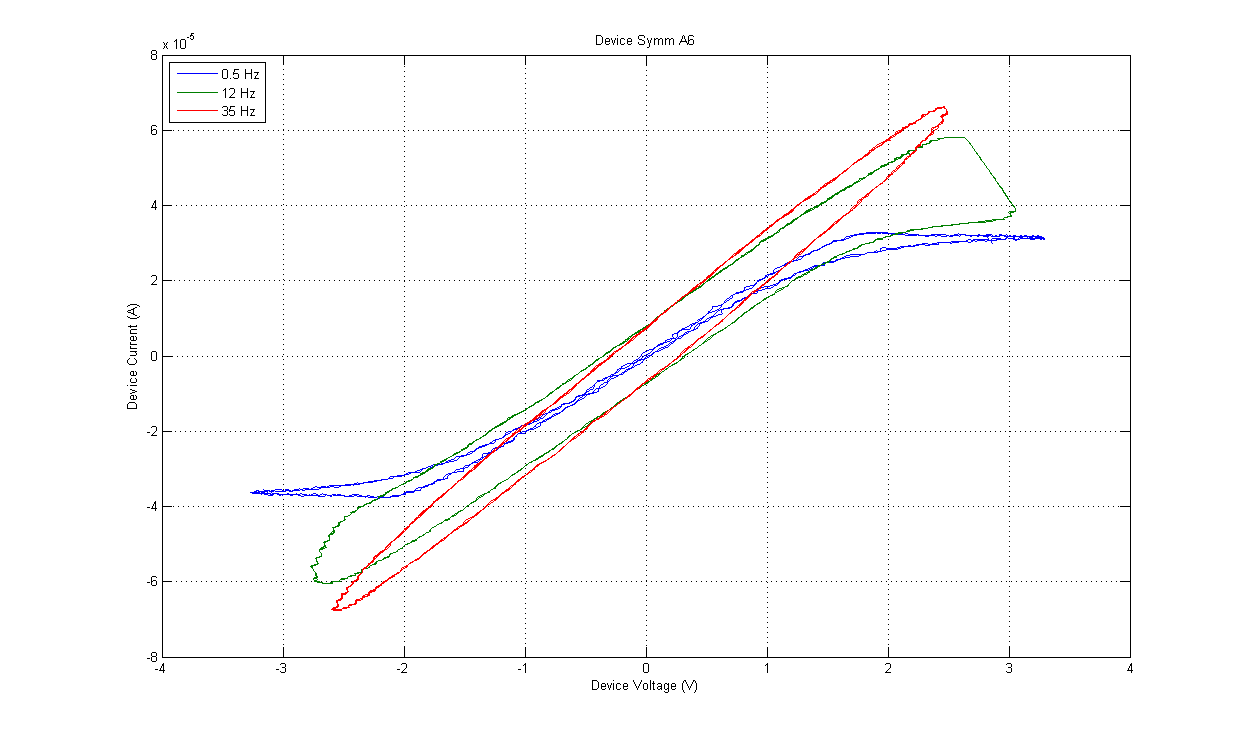
\includegraphics[scale=0.35]{experimental}
\caption{} 
\label{}
\end{figure}

\begin{figure}[!htp]
\centering
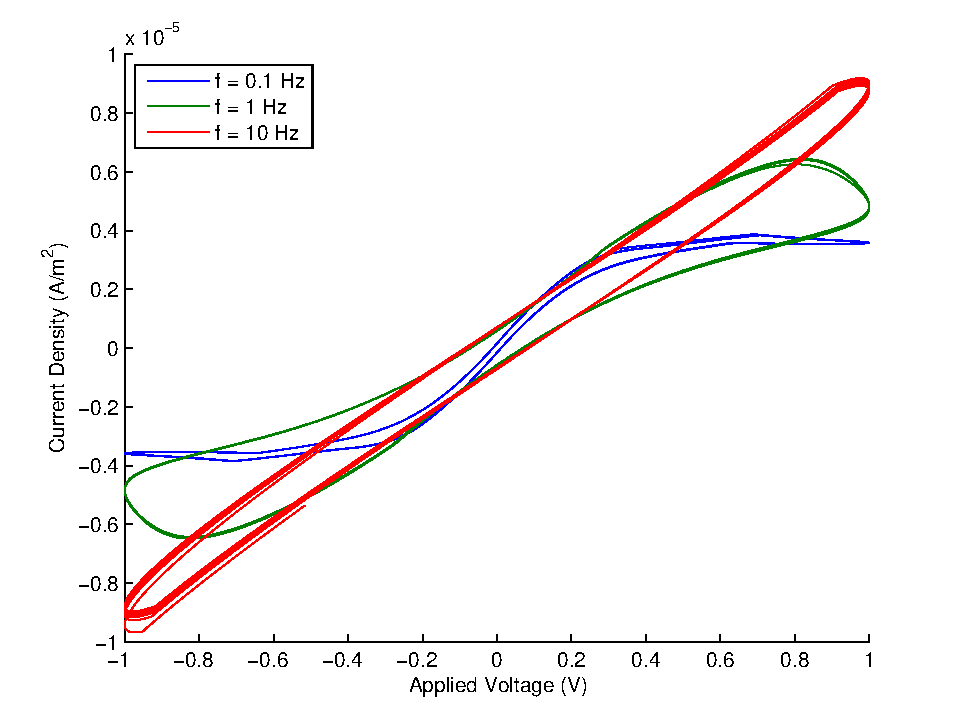
\includegraphics[scale=0.65]{MemF}
\caption{} 
\label{}
\end{figure}

\clearpage
\begin{figure}[!htp]
\centering
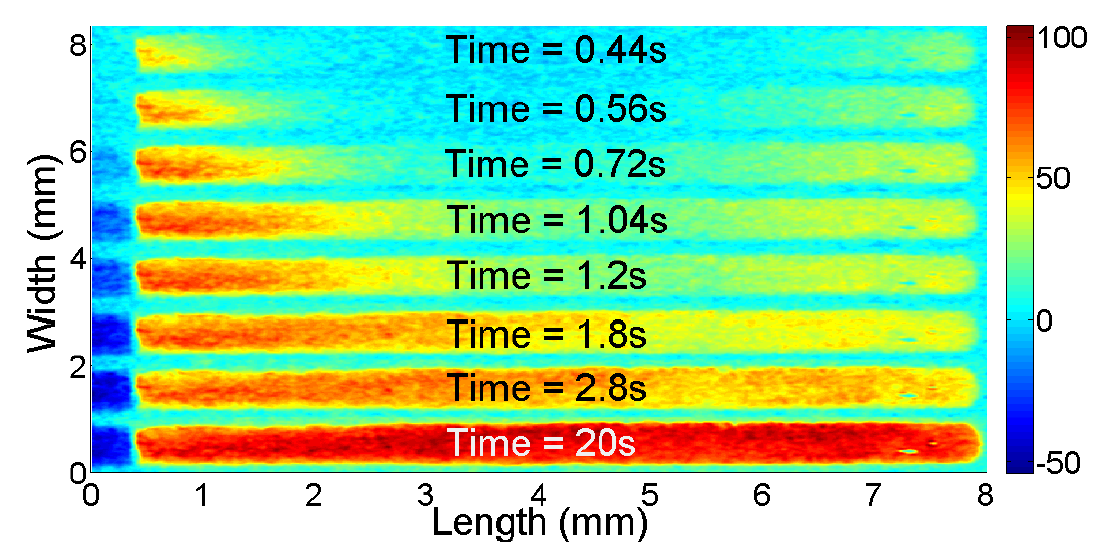
\includegraphics[scale=0.45]{notch}
\caption{} 
\label{}
\end{figure}

\begin{figure}[!htp]
\centering
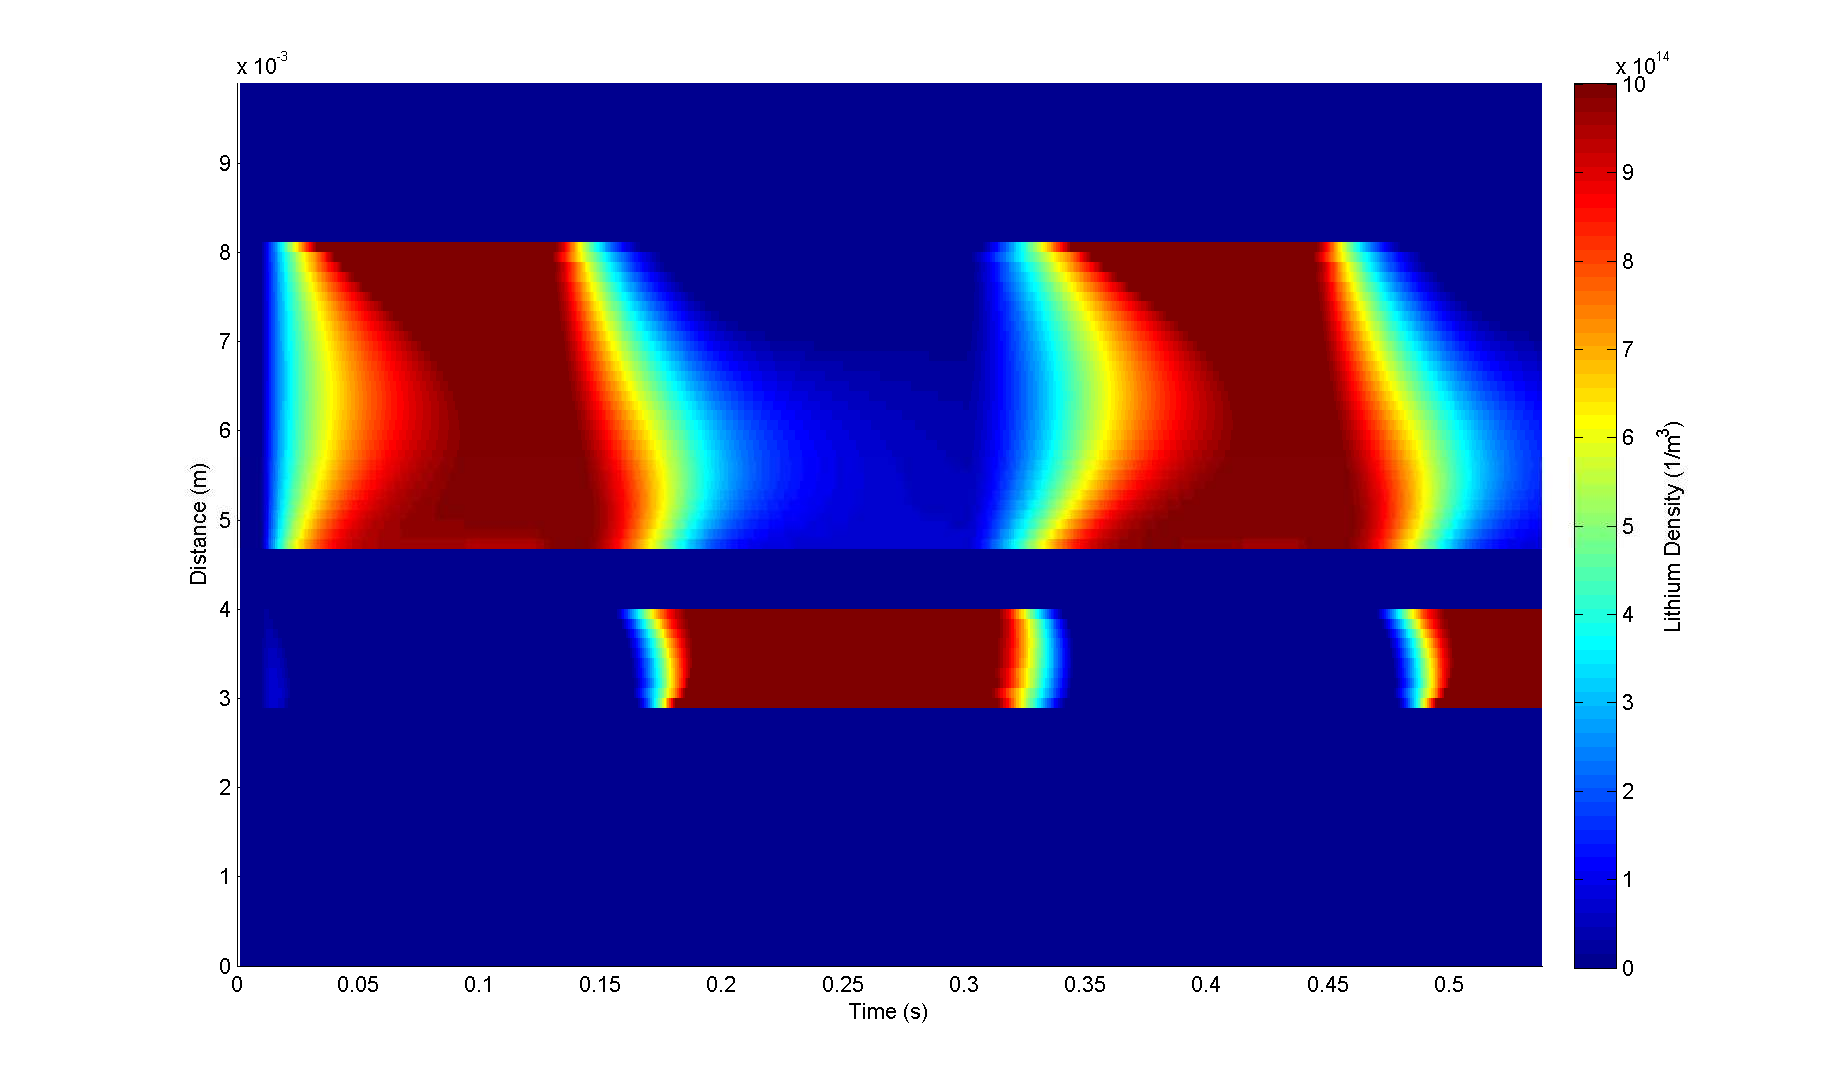
\includegraphics[scale=0.45]{Notch_flip_side}
\caption{} 
\label{}
\end{figure}


\end{doublespace}

